\addcontentsline{toc}{chapter}{Luke}
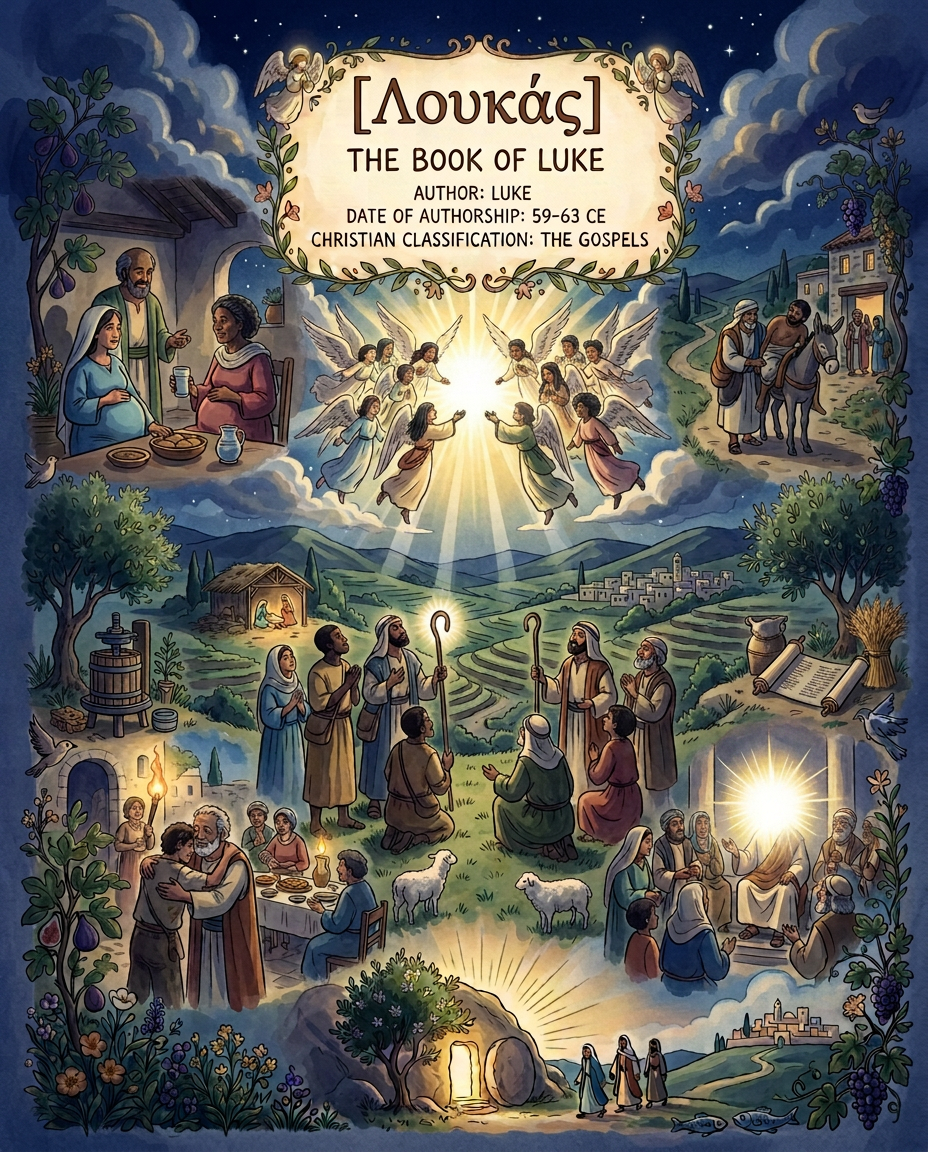
\includepdf[pages=1, fitpaper=false, width=\paperwidth, height=\paperheight, , keepaspectratio=false]{images/divider2/luke2.png}
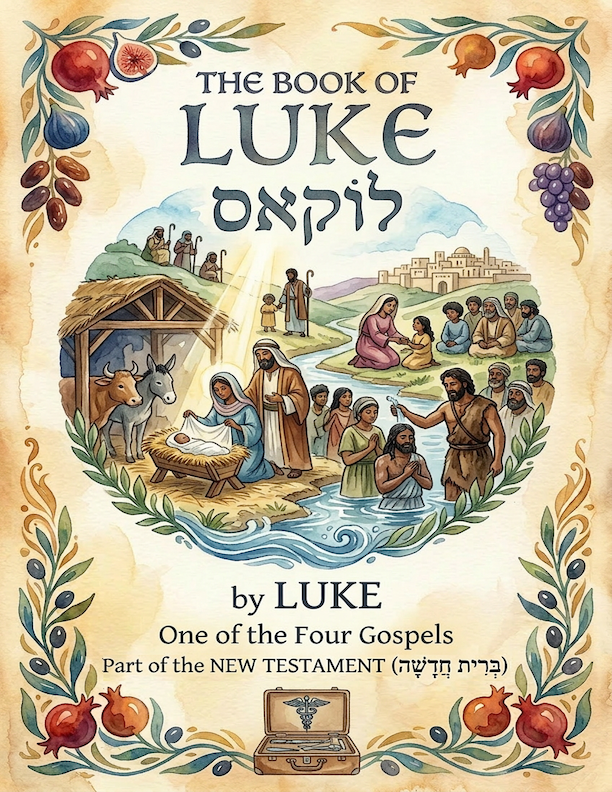
\includepdf[pages=1, fitpaper=false, width=\paperwidth, height=\paperheight, , keepaspectratio=false]{images/divider1/luke.png}

\includepdf[pages=1, fitpaper=false, width=\paperwidth, height=\paperheight, , keepaspectratio=false]{images/8.5x11-Dot-Grid.png}

\includepdf[pages=1, fitpaper=false, width=\paperwidth, height=\paperheight, , keepaspectratio=false]{images/8.5x11-Dot-Grid.png}


\mybook{Luke}
\vspace{-1.36in}


\mychapter{} \myverse*{}Since many have undertaken to set in order a narrative concerning
those matters which have been fulfilled among us,
\myverse{}even as those who from the beginning were eyewitnesses and servants of the word
delivered them to us,
\myverse{}it seemed good to me also, having traced the course of all things accurately
from the first, to write to you in order, most excellent Theophilus;
\myverse{}that you might know the certainty concerning the things in which you were instructed.

\myverse{}There was in the days of Herod, the king of Judea, a certain priest
named Zechariah, of the priestly division of Abijah. He had a wife of the daughters of Aaron, and her
name was Elisheva.
\myverse{}They were both righteous before God, walking blamelessly in all the commandments
and ordinances of the Lord.
\myverse{}But they had no child, because Elisheva was barren, and they both were well
advanced in years.

\myverse{}Now while he executed the priest’s office before God in the order
of his division
\myverse{}according to the custom of the priest’s office, his lot was to enter into the
temple of the Lord and burn incense.
\myverse{}The whole multitude of the people were praying outside at the hour of incense.

\myverse{}An angel of the Lord appeared to him, standing on the right side
of the altar of incense.
\myverse{}Zechariah was troubled when he saw him, and fear fell upon him.
\myverse{}But the angel said to him, “Don’t be afraid, Zechariah, because your request
has been heard. Your wife, Elisheva, will bear you a son, and you shall call his name Yochanan.
\myverse{}You will have joy and gladness, and many will rejoice at his birth.
\myverse{}For he will be great in the sight of the Lord, and he will drink no wine nor
strong drink. He will be filled with the Holy Spirit, even from his mother’s womb.
\myverse{}He will turn many of the children of Israel to the Lord their God.
\myverse{}He will go before him in the spirit and power of Elijah, ‘to turn the hearts
of the fathers to the children,’\footnote{ 1:17 Malachi 4:6} and the disobedient to the wisdom of the just;
to prepare a people prepared for the Lord.”

\myverse{}Zechariah said to the angel, “How can I be sure of this? For
I am an old man, and my wife is well advanced in years.”

\myverse{}The angel answered him, “I am Gabriel, who stands in the presence
of God. I was sent to speak to you and to bring you this good news.
\myverse{}Behold,\footnote{1:20 “Behold”, from “ἰδοὺ”, means look at, take notice, observe, see, or gaze at. It is often used
	as an interjection.} you will be silent and not able to speak until the day that these things
will happen, because you didn’t believe my words, which will be fulfilled in their proper time.”

\myverse{}The people were waiting for Zechariah, and they marveled that
he delayed in the temple.
\myverse{}When he came out, he could not speak to them. They perceived that he had seen
a vision in the temple. He continued making signs to them, and remained mute.
\myverse{}When the days of his service were fulfilled, he departed to his house.
\myverse{}After these days Elisheva his wife conceived, and she hid herself five months,
saying,
\myverse{}“Thus has the Lord done to me in the days in which he looked at me, to take
away my reproach among men.”

\myverse{}Now in the sixth month, the angel Gabriel was sent from God to
a city of Galilee named Nazareth,
\myverse{}to a virgin pledged to be married to a man whose name was Joseph, of David’s
house. The virgin’s name was Miriam.
\myverse{}Having come in, the angel said to her, “Rejoice, you highly favored one! The
Lord is with you. Blessed are you among women!”

\myverse{}But when she saw him, she was greatly troubled at the saying,
and considered what kind of salutation this might be.
\myverse{}The angel said to her, “Don’t be afraid, Miriam, for you have found favor
with God.
\myverse{}Behold, you will conceive in your womb and give birth to a son, and shall
name him ‘Yeshua.’
\myverse{}He will be great and will be called the Son of the Most High. The Lord God
will give him the throne of his father David,
\myverse{}and he will reign over the house of Jacob forever. There will be no end to
his Kingdom.”

\myverse{}Miriam said to the angel, “How can this be, seeing I am a virgin?”

\myverse{}The angel answered her, “The Holy Spirit will come on you, and
the power of the Most High will overshadow you. Therefore also the holy one who is born from you will
be called the Son of God.
\myverse{}Behold, Elisheva your relative also has conceived a son in her old age; and
this is the sixth month with her who was called barren.
\myverse{}For nothing spoken by God is impossible.”\footnote{1:37 or, “For everything spoken by God is possible.”}

\myverse{}Miriam said, “Behold, the servant of the Lord; let it be done
to me according to your word.”

Then the angel departed from her.

\myverse{}Miriam arose in those days and went into the hill country with
haste, into a city of Judah,
\myverse{}and entered into the house of Zechariah and greeted Elisheva.
\myverse{}When Elisheva heard Miriam’s greeting, the baby leaped in her womb; and Elisheva
was filled with the Holy Spirit.
\myverse{}She called out with a loud voice and said, “Blessed are you among women, and
blessed is the fruit of your womb!
\myverse{}Why am I so favored, that the mother of my Lord should come to me?
\myverse{}For behold, when the voice of your greeting came into my ears, the baby leaped
in my womb for joy!
\myverse{}Blessed is she who believed, for there will be a fulfillment of the things
which have been spoken to her from the Lord!”

\myverse{}Miriam said,

“My soul magnifies the Lord.

\myverse{}My spirit has rejoiced in God my Savior,

\myverse{}for he has looked at the humble state of his servant.

For behold, from now on, all generations will call me blessed.

\myverse{}For he who is mighty has done great things for me.

Holy is his name.

\myverse{}His mercy is for generations and generations on those
who fear him.

\myverse{}He has shown strength with his arm.

He has scattered the proud in the imagination of their hearts.

\myverse{}He has put down princes from their thrones,

and has exalted the lowly.

\myverse{}He has filled the hungry with good things.

He has sent the rich away empty.

\myverse{}He has given help to Israel, his servant, that he might remember
mercy,

\myverse{}as he spoke to our fathers,

to Abraham and his offspring\footnote{1:55 or, seed} forever.”

\myverse{}Miriam stayed with her about three months, and then returned
to her house.

\myverse{}Now the time that Elisheva should give birth was fulfilled, and
she gave birth to a son.
\myverse{}Her neighbors and her relatives heard that the Lord had magnified his mercy
toward her, and they rejoiced with her.
\myverse{}On the eighth day, they came to circumcise the child; and they would have
called him Zechariah, after the name of his father.
\myverse{}His mother answered, “Not so; but he will be called Yochanan.”

\myverse{}They said to her, “There is no one among your relatives who is
called by this name.”
\myverse{}They made signs to his father, what he would have him called.

\myverse{}He asked for a writing tablet, and wrote, “His name is Yochanan.”

They all marveled.
\myverse{}His mouth was opened immediately and his tongue freed, and he spoke, blessing
God.
\myverse{}Fear came on all who lived around them, and all these sayings were talked
about throughout all the hill country of Judea.
\myverse{}All who heard them laid them up in their heart, saying, “What then will this
child be?” The hand of the Lord was with him.

\myverse{}His father Zechariah was filled with the Holy Spirit, and prophesied,
saying,

\myverse{}“Blessed be the Lord, the God of Israel,

for he has visited and redeemed his people;

\myverse{}and has raised up a horn of salvation for us in the house of
his servant David

\myverse{}(as he spoke by the mouth of his holy prophets who
have been from of old),

\myverse{}salvation from our enemies and from the hand of all
who hate us;

\myverse{}to show mercy toward our fathers,

to remember his holy covenant,

\myverse{}the oath which he swore to Abraham our father,

\myverse{}to grant to us that we, being delivered out of the
hand of our enemies,

should serve him without fear,

\myverse{}in holiness and righteousness before him all the days
of our life.

\myverse{}And you, child, will be called a prophet of the Most High;

for you will go before the face of the Lord to prepare his ways,

\myverse{}to give knowledge of salvation to his people by the
remission of their sins,

\myverse{}because of the tender mercy of our God,

by which the dawn from on high will visit us,

\myverse{}to shine on those who sit in darkness and the shadow
of death;

to guide our feet into the way of peace.”

\myverse{}The child was growing and becoming strong in spirit, and was
in the desert until the day of his public appearance to Israel.


% LUKE 2
\mychapter{} \myverse*{}Now in those days, a decree went out from Caesar Augustus that
all the world should be enrolled.
\myverse{}This was the first enrollment made when Quirinius was governor of Syria.
\myverse{}All went to enroll themselves, everyone to his own city.
\myverse{}Joseph also went up from Galilee, out of the city of Nazareth, into Judea, to
David’s city, which is called Bethlehem, because he was of the house and family of David,
\myverse{}to enroll himself with Miriam, who was pledged to be married to him as wife,
being pregnant.

\myverse{}While they were there, the day had come for her to give birth.
\myverse{}She gave birth to her firstborn son. She wrapped him in bands of cloth and laid
him in a feeding trough, because there was no room for them in the inn.

\myverse{}There were shepherds in the same country staying in the field,
and keeping watch by night over their flock.
\myverse{}Behold, an angel of the Lord stood by them, and the glory of the Lord shone
around them, and they were terrified.
\myverse{}The angel said to them, “Don’t be afraid, for behold, I bring you good news
of great joy which will be to all the people.
\myverse{}For there is born to you today, in David’s city, a Savior, who is Messiah\footnote{2:11 “Messiah” means “Anointed One”.} the Lord.
\myverse{}This is the sign to you: you will find a baby wrapped in strips of cloth,
lying in a feeding trough.”
\myverse{}Suddenly, there was with the angel a multitude of the heavenly army praising
God and saying,

\myverse{}“Glory to God in the highest,

on earth peace, good will toward men.”

\myverse{}When the angels went away from them into the sky, the shepherds
said to one another, “Let’s go to Bethlehem, now, and see this thing that has happened, which the Lord
has made known to us.”
\myverse{}They came with haste and found both Miriam and Joseph, and the baby was lying
in the feeding trough.
\myverse{}When they saw it, they publicized widely the saying which was spoken to them
about this child.
\myverse{}All who heard it wondered at the things which were spoken to them by the shepherds.
\myverse{}But Miriam kept all these sayings, pondering them in her heart.
\myverse{}The shepherds returned, glorifying and praising God for all the things that
they had heard and seen, just as it was told them.

\myverse{}When eight days were fulfilled for the circumcision of the child,
his name was called Yeshua, which was given by the angel before he was conceived in the womb.

\myverse{}When the days of their purification according to the Torah of Moses
were fulfilled, they brought him up to Jerusalem to present him to the Lord
\myverse{}(as it is written in the Torah of the Lord, “Every male who opens the womb
shall be called holy to the Lord”),\footnote{ 2:23 Exodus 13:2,12}
\myverse{}and to offer a sacrifice according to that which is said in the Torah of the Lord,
“A pair of turtledoves, or two young pigeons.”\footnote{ 2:24 Leviticus 12:8}

\myverse{}Behold, there was a man in Jerusalem whose name was Simeon. This
man was righteous and devout, looking for the consolation of Israel, and the Holy Spirit was on him.
\myverse{}It had been revealed to him by the Holy Spirit that he should not see death
before he had seen the Lord’s Messiah.\footnote{2:26 “Christ” (Greek) and “Messiah” (Hebrew) both mean “Anointed One”}
\myverse{}He came in the Spirit into the temple. When the parents brought in the child,
Yeshua, that they might do concerning him according to the requirement of the Torah,
\myverse{}then he received him into his arms and blessed God, and said,

\myverse{}“Now you are releasing your servant, Master,

according to your word, in peace;

\myverse{}for my eyes have seen your salvation,

\myverse{}which you have prepared before the face of all peoples;

\myverse{}a light for revelation to the nations,

and the glory of your people Israel.”

\myverse{}Joseph and his mother were marveling at the things which were
spoken concerning him.
\myverse{}Simeon blessed them, and said to Miriam, his mother, “Behold, this child is
appointed for the falling and the rising of many in Israel, and for a sign which is spoken against.
\myverse{}Yes, a sword will pierce through your own soul, that the thoughts of many
hearts may be revealed.”

\myverse{}There was one Hannah, a prophetess, the daughter of Penuel, of
the tribe of Asher (she was of a great age, having lived with a husband seven years from her virginity,
\myverse{}and she had been a widow for about eighty-four years), who didn’t depart from
the temple, worshiping with fastings and petitions night and day.
\myverse{}Coming up at that very hour, she gave thanks to the Lord, and spoke of him
to all those who were looking for redemption in Jerusalem.

\myverse{}When they had accomplished all things that were according to
the Torah of the Lord, they returned into Galilee, to their own city, Nazareth.
\myverse{}The child was growing, and was becoming strong in spirit, being filled with
wisdom, and the grace of God was upon him.

\myverse{}His parents went every year to Jerusalem at the feast of the
Passover.
\myverse{}When he was twelve years old, they went up to Jerusalem according to the custom
of the feast;
\myverse{}and when they had fulfilled the days, as they were returning, the boy Yeshua
stayed behind in Jerusalem. Joseph and his mother didn’t know it,
\myverse{}but supposing him to be in the company, they went a day’s journey; and they
looked for him among their relatives and acquaintances.
\myverse{}When they didn’t find him, they returned to Jerusalem, looking for him.
\myverse{}After three days they found him in the temple, sitting in the middle of the
teachers, both listening to them and asking them questions.
\myverse{}All who heard him were amazed at his understanding and his answers.
\myverse{}When they saw him, they were astonished; and his mother said to him, “Son,
why have you treated us this way? Behold, your father and I were anxiously looking for you.”

\myverse{}He said to them,
\textcolor{crimson}{“Why were you looking for me? Didn’t you know that I must be in my Father’s house?”}
\myverse{}They didn’t understand the saying which he spoke to them.
\myverse{}And he went down with them and came to Nazareth. He was subject to them, and
his mother kept all these sayings in her heart.
\myverse{}And Yeshua increased in wisdom and stature, and in favor with God and men.


% LUKE 3
\mychapter{} \myverse*{}Now in the fifteenth year of the reign of Tiberius Caesar, Pontius
Pilate being governor of Judea, and Herod being tetrarch of Galilee, and his brother Philip tetrarch of
the region of Ituraea and Trachonitis, and Lysanias tetrarch of Abilene,
\myverse{}during the high priesthood of Annas and Caiaphas, the word of God came to Yochanan,
the son of Zechariah, in the wilderness.
\myverse{}He came into all the region around the Jordan, proclaiming the immersion of
repentance for remission of sins.
\myverse{}As it is written in the scroll of the words of Isaiah the prophet,

“The voice of one crying in the wilderness,

‘Make ready the way of the Lord.

Make his paths straight.

\myverse{}Every valley will be filled.

Every mountain and hill will be brought low.

The crooked will become straight,

and the rough ways smooth.

\myverse{}All flesh will see God’s salvation.’ ”\footnote{ 3:6 Isaiah 40:3-5}

\myverse{}He said therefore to the multitudes who went out to be immersed
by him, “You offspring of vipers, who warned you to flee from the wrath to come?
\myverse{}Therefore produce fruits worthy of repentance, and don’t begin to say among
yourselves, ‘We have Abraham for our father;’ for I tell you that God is able to raise up children to
Abraham from these stones!
\myverse{}Even now the ax also lies at the root of the trees. Every tree therefore that
doesn’t produce good fruit is cut down and thrown into the fire.”

\myverse{}The multitudes asked him, “What then must we do?”

\myverse{}He answered them, “He who has two coats, let him give to him
who has none. He who has food, let him do likewise.”

\myverse{}Tax collectors also came to be immersed, and they said to him,
“Rabbi, what must we do?”

\myverse{}He said to them, “Collect no more than that which is appointed
to you.”

\myverse{}Soldiers also asked him, saying, “What about us? What must we
do?”

He said to them, “Extort from no one by violence, neither accuse anyone wrongfully. Be content
with your wages.”

\myverse{}As the people were in expectation, and all men reasoned in their
hearts concerning Yochanan, whether perhaps he was the Messiah,
\myverse{}Yochanan answered them all, “I indeed immerse you with water, but he comes
who is mightier than I, the strap of whose sandals I am not worthy to loosen. He will immerse you in the
Holy Spirit and fire.
\myverse{}His winnowing fan is in his hand, and he will thoroughly cleanse his threshing
floor, and will gather the wheat into his barn; but he will burn up the chaff with unquenchable fire.”

\myverse{}Then with many other exhortations he preached good news to the
people,
\myverse{}but Herod the tetrarch,\footnote{3:19 a tetrarch is one of four governors of a province} being reproved by him for Herodias,
his brother’s\footnote{3:19 TR reads “brother Philip’s” instead of “brother’s”} wife, and for all the evil things
which Herod had done,
\myverse{}added this also to them all, that he shut up Yochanan in prison.

\myverse{}Now when all the people were immersed, Yeshua also had been immersed
and was praying. The sky was opened,
\myverse{}and the Holy Spirit descended in a bodily form like a dove on him; and a voice
came out of the sky, saying “You are my beloved Son. In you I am well pleased.”

\myverse{}Yeshua himself, when he began to teach, was about thirty years
old, being the son (as was supposed) of Joseph, the son of Eli,
\myverse{}the son of Matthat, the son of Levi, the son of Melchi, the son of Jannai,
the son of Joseph,
\myverse{}the son of Mattithiah, the son of Amos, the son of Nahum, the son of Esli,
the son of Naggai,
\myverse{}the son of Maath, the son of Mattithiah, the son of Shimei, the son of Joseph,
the son of Judah,
\myverse{}the son of Yochanan, the son of Rhesa, the son of Zerubbabel, the son of Shealtiel,
the son of Neri,
\myverse{}the son of Melchi, the son of Addi, the son of Cosam, the son of Elmodam,
the son of Er,
\myverse{}the son of Yosi, the son of Eliezer, the son of Jorim, the son of Matthat,
the son of Levi,
\myverse{}the son of Simeon, the son of Judah, the son of Joseph, the son of Jonan,
the son of Eliakim,
\myverse{}the son of Maleah, the son of Manah, the son of Mattathah, the son of Nathan,
the son of David,
\myverse{}the son of Jesse, the son of Obed, the son of Boaz, the son of Salmon, the
son of Nahshon,
\myverse{}the son of Amminadab, the son of Ram,\footnote{3:33 NU reads “Admin, the son of Arni” instead of “Ram”} the son of Hezron, the son of Perez,
the son of Judah,
\myverse{}the son of Jacob, the son of Isaac, the son of Abraham, the son of Terah,
the son of Nahor,
\myverse{}the son of Serug, the son of Reu, the son of Peleg, the son of Eber, the son
of Shelah,
\myverse{}the son of Kenan, the son of Arpachshad, the son of Shem, the son of Noah,
the son of Lamech,
\myverse{}the son of Methuselah, the son of Enoch, the son of Jared, the son of Mahalalel,
the son of Kenan,
\myverse{}the son of Enosh, the son of Seth, the son of Adam, the son of God.


% LUKE 4
\mychapter{} \myverse*{}Yeshua, full of the Holy Spirit, returned from the Jordan and was
led by the Spirit into the wilderness
\myverse{}for forty days, being tempted by the devil. He ate nothing in those days. Afterward,
when they were completed, he was hungry.

\myverse{}The devil said to him, “If you are the Son of God, command this
stone to become bread.”

\myverse{}Yeshua answered him, saying,
\textcolor{crimson}{“It is written, ‘Man shall not live by bread alone, but by every word of God.’ ”}\footnote{ 4:4 Deuteronomy 8:3}

\myverse{}The devil, leading him up on a high mountain, showed him all the
kingdoms of the world in a moment of time.
\myverse{}The devil said to him, “I will give you all this authority and their glory,
for it has been delivered to me, and I give it to whomever I want.
\myverse{}If you therefore will worship before me, it will all be yours.”

\myverse{}Yeshua answered him,
\textcolor{crimson}{“Get behind me, Satan! For it is written, ‘You shall worship the Lord your God, and you shall serve
	him only.’ ”}\footnote{ 4:8 Deuteronomy 6:13}

\myverse{}He led him to Jerusalem and set him on the pinnacle of the temple,
and said to him, “If you are the Son of God, cast yourself down from here,
\myverse{}for it is written,

‘He will put his angels in charge of you, to guard you;’

\myverse{}and,

‘On their hands they will bear you up,

lest perhaps you dash your foot against a stone.’ ”\footnote{ 4:11 Psalms 91:11-12
}

\myverse{}Yeshua answering, said to him,
\textcolor{crimson}{“It has been said, ‘You shall not tempt the Lord your God.’ ”}\footnote{ 4:12 Deuteronomy 6:16}

\myverse{}When the devil had completed every temptation, he departed from
him until another time.

\myverse{}Yeshua returned in the power of the Spirit into Galilee, and
news about him spread through all the surrounding area.
\myverse{}He taught in their synagogues, being glorified by all.

\myverse{}He came to Nazareth, where he had been brought up. He entered,
as was his custom, into the synagogue on the Sabbath day, and stood up to read.
\myverse{}The scroll of the prophet Isaiah was handed to him. He opened the scroll,
and found the place where it was written,

\myverse{}\textcolor{crimson}{“The Spirit of the Lord is on me,}

\textcolor{crimson}{because he has anointed me to proclaim good news to the poor.}

\textcolor{crimson}{He has sent me to heal the broken hearted,}\footnote{4:18 NU omits “to heal the broken hearted”}

\textcolor{crimson}{to proclaim release to the captives,}

\textcolor{crimson}{recovering of sight to the blind,}

\textcolor{crimson}{to deliver those who are crushed,}

\myverse{}\textcolor{crimson}{and to proclaim the acceptable year of the Lord.”}\footnote{ 4:19 Isaiah 61:1-2}

\myverse{}He closed the scroll, gave it back to the shammash, and sat down.
The eyes of all in the synagogue were fastened on him.
\myverse{}He began to tell them,
\textcolor{crimson}{“Today, this Scripture has been fulfilled in your hearing.”}

\myverse{}All testified about him and wondered at the gracious words which
proceeded out of his mouth; and they said, “Isn’t this Joseph’s son?”

\myverse{}He said to them,
\textcolor{crimson}{“Doubtless you will tell me this proverb, ‘Physician, heal yourself! Whatever we have heard done at
	Capernaum, do also here in your hometown.’ ”}
\myverse{}He said,
\textcolor{crimson}{“Most certainly I tell you, no prophet is acceptable in his hometown.
}
\myverse{}\textcolor{crimson}{But truly I tell you, there were many widows in Israel in the days of
	Elijah, when the sky was shut up three years and six months, when a great famine came over all the land.
}
\myverse{}\textcolor{crimson}{Elijah was sent to none of them, except to Zarephath, in the land of Sidon,
	to a woman who was a widow.
}
\myverse{}\textcolor{crimson}{There were many lepers in Israel in the time of Elisha the prophet, yet
	not one of them was cleansed, except Naaman, the Syrian.”}

\myverse{}They were all filled with wrath in the synagogue as they heard
these things.
\myverse{}They rose up, threw him out of the city, and led him to the brow of the hill
that their city was built on, that they might throw him off the cliff.
\myverse{}But he, passing through the middle of them, went his way.

\myverse{}He came down to Capernaum, a city of Galilee. He was teaching
them on the Sabbath day,
\myverse{}and they were astonished at his teaching, for his word was with authority.
\myverse{}In the synagogue there was a man who had a spirit of an unclean demon; and
he cried out with a loud voice,
\myverse{}saying, “Ah! what have we to do with you, Yeshua of Nazareth? Have you come
to destroy us? I know who you are: the Holy One of God!”

\myverse{}Yeshua rebuked him, saying,
\textcolor{crimson}{“Be silent and come out of him!”
} When the demon had thrown him down in the middle of them, he came out of him, having done him no
harm.

\myverse{}Amazement came on all and they spoke together, one with another,
saying, “What is this word? For with authority and power he commands the unclean spirits, and they come
out!”
\myverse{}News about him went out into every place of the surrounding region.

\myverse{}He rose up from the synagogue and entered into Simon’s house.
Simon’s mother-in-law was afflicted with a great fever, and they begged him to help her.
\myverse{}He stood over her and rebuked the fever, and it left her. Immediately she
rose up and served them.
\myverse{}When the sun was setting, all those who had any sick with various diseases
brought them to him; and he laid his hands on every one of them, and healed them.
\myverse{}Demons also came out of many, crying out and saying, “You are the Messiah,
the Son of God!” Rebuking them, he didn’t allow them to speak, because they knew that he was the Messiah.

\myverse{}When it was day, he departed and went into an uninhabited place
and the multitudes looked for him, and came to him, and held on to him, so that he wouldn’t go away from
them.
\myverse{}But he said to them,
\textcolor{crimson}{“I must proclaim the good news of God’s Kingdom to the other cities also. For this reason I have been
	sent.”}
\myverse{}He was proclaiming in the synagogues of Galilee.


% LUKE 5
\mychapter{} \myverse*{}Now while the multitude pressed on him and heard the word of God,
he was standing by the lake of Gennesaret.
\myverse{}He saw two boats standing by the lake, but the fishermen had gone out of them
and were washing their nets.
\myverse{}He entered into one of the boats, which was Simon’s, and asked him to put out
a little from the land. He sat down and taught the multitudes from the boat.

\myverse{}When he had finished speaking, he said to Simon,
\textcolor{crimson}{“Put out into the deep and let down your nets for a catch.”}

\myverse{}Simon answered him, “Master, we worked all night and caught nothing;
but at your word I will let down the net.”
\myverse{}When they had done this, they caught a great multitude of fish, and their net
was breaking.
\myverse{}They beckoned to their partners in the other boat, that they should come and
help them. They came and filled both boats, so that they began to sink.
\myverse{}But Simon Peter, when he saw it, fell down at Yeshua’s knees, saying, “Depart
from me, for I am a sinful man, Lord.”
\myverse{}For he was amazed, and all who were with him, at the catch of fish which they
had caught;
\myverse{}and so also were Jacob and Yochanan, sons of Zebedee, who were partners with
Simon.

Yeshua said to Simon,
\textcolor{crimson}{“Don’t be afraid. From now on you will be catching people alive.”}

\myverse{}When they had brought their boats to land, they left everything,
and followed him.

\myverse{}While he was in one of the cities, behold, there was a man full
of leprosy. When he saw Yeshua, he fell on his face and begged him, saying, “Lord, if you want to, you
can make me clean.”

\myverse{}He stretched out his hand and touched him, saying,
\textcolor{crimson}{“I want to. Be made clean.”}

Immediately the leprosy left him.
\myverse{}He commanded him to tell no one,
\textcolor{crimson}{“But go your way and show yourself to the priest, and offer for your cleansing according to what Moses
	commanded, for a testimony to them.”}

\myverse{}But the report concerning him spread much more, and great multitudes
came together to hear and to be healed by him of their infirmities.
\myverse{}But he withdrew himself into the desert and prayed.

\myverse{}On one of those days, he was teaching; and there were Pharisees
and teachers of the Torah sitting by who had come out of every village of Galilee, Judea, and Jerusalem.
The power of the Lord was with him to heal them.
\myverse{}Behold, men brought a paralyzed man on a cot, and they sought to bring him
in to lay before Yeshua.
\myverse{}Not finding a way to bring him in because of the multitude, they went up to
the housetop and let him down through the tiles with his cot into the middle before Yeshua.
\myverse{}Seeing their faith, he said to him,
\textcolor{crimson}{“Man, your sins are forgiven you.”}

\myverse{}The scribes and the Pharisees began to reason, saying, “Who is
this who speaks blasphemies? Who can forgive sins, but God alone?”

\myverse{}But Yeshua, perceiving their thoughts, answered them,
\textcolor{crimson}{“Why are you reasoning so in your hearts?
}
\myverse{}\textcolor{crimson}{Which is easier to say, ‘Your sins are forgiven you,’ or to say, ‘Arise
	and walk’?
}
\myverse{}\textcolor{crimson}{But that you may know that the Son of Man has authority on earth to forgive
	sins,”} he said to the paralyzed man,
\textcolor{crimson}{“I tell you, arise, take up your cot, and go to your house.”}

\myverse{}Immediately he rose up before them, and took up that which he
was laying on, and departed to his house, glorifying God.
\myverse{}Amazement took hold on all, and they glorified God. They were filled with
fear, saying, “We have seen strange things today.”

\myverse{}After these things he went out and saw a tax collector named
Levi sitting at the tax office, and said to him,
\textcolor{crimson}{“Follow me!”}

\myverse{}He left everything, and rose up and followed him.
\myverse{}Levi made a great feast for him in his house. There was a great crowd of tax
collectors and others who were reclining with them.
\myverse{}Their scribes and the Pharisees murmured against his disciples, saying, “Why
do you eat and drink with the tax collectors and sinners?”

\myverse{}Yeshua answered them,
\textcolor{crimson}{“Those who are healthy have no need for a physician, but those who are sick do.
}
\myverse{}\textcolor{crimson}{I have not come to call the righteous, but sinners, to repentance.”
}

\myverse{}They said to him, “Why do Yochanan’s disciples often fast and
pray, likewise also the disciples of the Pharisees, but yours eat and drink?”

\myverse{}He said to them,
\textcolor{crimson}{“Can you make the friends of the bridegroom fast while the bridegroom is with them?
}
\myverse{}\textcolor{crimson}{But the days will come when the bridegroom will be taken away from them.
	Then they will fast in those days.”}

\myverse{}He also told a parable to them.
\textcolor{crimson}{“No one puts a piece from a new garment on an old garment, or else he will tear the new, and also
	the piece from the new will not match the old.
}
\myverse{}\textcolor{crimson}{No one puts new wine into old wineskins, or else the new wine will burst
	the skins, and it will be spilled and the skins will be destroyed.
}
\myverse{}\textcolor{crimson}{But new wine must be put into fresh wineskins, and both are preserved.
}
\myverse{}\textcolor{crimson}{No man having drunk old wine immediately desires new, for he says, ‘The
	old is better.’ ”}


% LUKE 6
\mychapter{} \myverse*{}Now on the second Sabbath after the first, he was going through
the grain fields. His disciples plucked the heads of grain and ate, rubbing them in their hands.
\myverse{}But some of the Pharisees said to them, “Why do you do that which is not lawful
to do on the Sabbath day?”

\myverse{}Yeshua, answering them, said,
\textcolor{crimson}{“Haven’t you read what David did when he was hungry, he and those who were with him,
}
\myverse{}\textcolor{crimson}{how he entered into God’s house, and took and ate the show bread, and gave
	also to those who were with him, which is not lawful to eat except for the priests alone?”}
\myverse{}He said to them,
\textcolor{crimson}{“The Son of Man is lord of the Sabbath.”}

\myverse{}It also happened on another Sabbath that he entered into the synagogue
and taught. There was a man there, and his right hand was withered.
\myverse{}The scribes and the Pharisees watched him, to see whether he would heal on the
Sabbath, that they might find an accusation against him.
\myverse{}But he knew their thoughts; and he said to the man who had the withered hand,
\textcolor{crimson}{“Rise up and stand in the middle.”} He arose and stood.
\myverse{}Then Yeshua said to them,
\textcolor{crimson}{“I will ask you something: Is it lawful on the Sabbath to do good, or to do harm? To save a life,
	or to kill?”}
\myverse{}He looked around at them all, and said to the man,
\textcolor{crimson}{“Stretch out your hand.”} He did, and his hand was restored as sound as the other.
\myverse{}But they were filled with rage, and talked with one another about what they
might do to Yeshua.

\myverse{}In these days, he went out to the mountain to pray, and he continued
all night in prayer to God.
\myverse{}When it was day, he called his disciples, and from them he chose twelve, whom
he also named emissaries:
\myverse{}Simon, whom he also named Peter; Andrew, his brother; Jacob; Yochanan; Philip;
Bartholomew;
\myverse{}Matthew; Thomas; Jacob the son of Halfai; Simon who was called the Zealot;
\myverse{}Judah the son of Jacob; and Judah Iscariot, who also became a traitor.

\myverse{}He came down with them and stood on a level place, with a crowd
of his disciples and a great number of the people from all Judea and Jerusalem and the sea coast of Tyre
and Sidon, who came to hear him and to be healed of their diseases,
\myverse{}as well as those who were troubled by unclean spirits; and they were being
healed.
\myverse{}All the multitude sought to touch him, for power came out of him and healed
them all.

\myverse{}He lifted up his eyes to his disciples, and said:

\textcolor{crimson}{“Blessed are you who are poor,}

\textcolor{crimson}{for God’s Kingdom is yours.}

\myverse{}\textcolor{crimson}{Blessed are you who hunger now,}

\textcolor{crimson}{for you will be filled.}

\textcolor{crimson}{Blessed are you who weep now,}

\textcolor{crimson}{for you will laugh.}

\myverse{}\textcolor{crimson}{Blessed are you when men hate you, and when they exclude
	and mock you, and throw out your name as evil, for the Son of Man’s sake.
}

\myverse{}\textcolor{crimson}{Rejoice in that day and leap for joy, for behold,
	your reward is great in heaven, for their fathers did the same thing to the prophets.}


\vspace{\baselineskip} \myverse{}\textcolor{crimson}{“But woe to you who are rich!}

\textcolor{crimson}{For you have received your consolation.}

\myverse{}\textcolor{crimson}{Woe to you, you who are full now,}

\textcolor{crimson}{for you will be hungry.}

\textcolor{crimson}{Woe to you who laugh now,}

\textcolor{crimson}{for you will mourn and weep.}

\myverse{}\textcolor{crimson}{Woe,}\footnote{6:26 TR adds “to you”}
\textcolor{crimson}{when}\footnote{6:26 TR adds “all”
}
\textcolor{crimson}{men speak well of you,}

\textcolor{crimson}{for their fathers did the same thing to the false prophets.}

\myverse{}\textcolor{crimson}{“But I tell you who hear: love your enemies, do good to those
	who hate you,
}
\myverse{}\textcolor{crimson}{bless those who curse you, and pray for those who mistreat you.
}
\myverse{}\textcolor{crimson}{To him who strikes you on the cheek, offer also the other; and from him
	who takes away your cloak, don’t withhold your coat also.
}
\myverse{}\textcolor{crimson}{Give to everyone who asks you, and don’t ask him who takes away your goods
	to give them back again.}

\myverse{}\textcolor{crimson}{“As you would like people to do to you, do exactly so to
	them.
}

\myverse{}\textcolor{crimson}{“If you love those who love you, what credit is that to you?
	For even sinners love those who love them.
}
\myverse{}\textcolor{crimson}{If you do good to those who do good to you, what credit is that to you?
	For even sinners do the same.
}
\myverse{}\textcolor{crimson}{If you lend to those from whom you hope to receive, what credit is that
	to you? Even sinners lend to sinners, to receive back as much.
}
\myverse{}\textcolor{crimson}{But love your enemies, and do good, and lend, expecting nothing back;
	and your reward will be great, and you will be children of the Most High; for he is kind toward the unthankful
	and evil.}

\myverse{}\textcolor{crimson}{“Therefore be merciful,}

\textcolor{crimson}{even as your Father is also merciful.}

\myverse{}\textcolor{crimson}{Don’t judge,}

\textcolor{crimson}{and you won’t be judged.}

\textcolor{crimson}{Don’t condemn,}

\textcolor{crimson}{and you won’t be condemned.}

\textcolor{crimson}{Set free,}

\textcolor{crimson}{and you will be set free.}

\myverse{}\textcolor{crimson}{“Give, and it will be given to you: good measure, pressed
	down, shaken together, and running over, will be given to you.}\footnote{6:38 literally, into your bosom.}
\textcolor{crimson}{For with the same measure you measure it will be measured back to you.”}

\myverse{}He spoke a parable to them.
\textcolor{crimson}{“Can the blind guide the blind? Won’t they both fall into a pit?
}
\myverse{}\textcolor{crimson}{A disciple is not above his rabbi, but everyone when he is fully trained
	will be like his rabbi.
}
\myverse{}\textcolor{crimson}{Why do you see the speck of chaff that is in your brother’s eye, but don’t
	consider the beam that is in your own eye?
}
\myverse{}\textcolor{crimson}{Or how can you tell your brother, ‘Brother, let me remove the speck of
	chaff that is in your eye,’ when you yourself don’t see the beam that is in your own eye? You hypocrite!
	First remove the beam from your own eye, and then you can see clearly to remove the speck of chaff that
	is in your brother’s eye.
}

\myverse{}\textcolor{crimson}{“For there is no good tree that produces rotten fruit, nor
	again a rotten tree that produces good fruit.
}
\myverse{}\textcolor{crimson}{For each tree is known by its own fruit. For people don’t gather figs
	from thorns, nor do they gather grapes from a bramble bush.
}
\myverse{}\textcolor{crimson}{The good man out of the good treasure of his heart brings out that which
	is good, and the evil man out of the evil treasure of his heart brings out that which is evil, for out
	of the abundance of the heart, his mouth speaks.}

\myverse{}\textcolor{crimson}{“Why do you call me, ‘Lord, Lord,’ and don’t do the things
	which I say?
}
\myverse{}\textcolor{crimson}{Everyone who comes to me, and hears my words and does them, I will show
	you who he is like.
}
\myverse{}\textcolor{crimson}{He is like a man building a house, who dug and went deep and laid a foundation
	on the rock. When a flood arose, the stream broke against that house, and could not shake it, because
	it was founded on the rock.
}
\myverse{}\textcolor{crimson}{But he who hears and doesn’t do, is like a man who built a house on the
	earth without a foundation, against which the stream broke, and immediately it fell; and the ruin of that
	house was great.”}


% LUKE 7
\mychapter{} \myverse*{}After he had finished speaking in the hearing of the people, he
entered into Capernaum.
\myverse{}A certain centurion’s servant, who was dear to him, was sick and at the point
of death.
\myverse{}When he heard about Yeshua, he sent to him Jewish elders, asking him to come
and save his servant.
\myverse{}When they came to Yeshua, they begged him earnestly, saying, “He is worthy for
you to do this for him,
\myverse{}for he loves our nation, and he built our synagogue for us.”
\myverse{}Yeshua went with them. When he was now not far from the house, the centurion
sent friends to him, saying to him, “Lord, don’t trouble yourself, for I am not worthy for you to come
under my roof.
\myverse{}Therefore I didn’t even think myself worthy to come to you; but say the word,
and my servant will be healed.
\myverse{}For I also am a man placed under authority, having under myself soldiers. I
tell this one, ‘Go!’ and he goes; and to another, ‘Come!’ and he comes; and to my servant, ‘Do this,’
and he does it.”

\myverse{}When Yeshua heard these things, he marveled at him, and turned
and said to the multitude who followed him,
\textcolor{crimson}{“I tell you, I have not found such great faith, no, not in Israel.”}
\myverse{}Those who were sent, returning to the house, found that the servant who had
been sick was well.

\myverse{}Soon afterwards, he went to a city called Nain. Many of his disciples,
along with a great multitude, went with him.
\myverse{}Now when he came near to the gate of the city, behold, one who was dead was
carried out, the only born\footnote{7:12 The phrase “only born” is from the Greek word “μονογενη”, which is sometimes translated “only
	begotten” or “one and only”.
} son of his mother, and she was a widow. Many people of the city were with her.
\myverse{}When the Lord saw her, he had compassion on her and said to her,
\textcolor{crimson}{“Don’t cry.”}
\myverse{}He came near and touched the coffin, and the bearers stood still. He said,
\textcolor{crimson}{“Young man, I tell you, arise!”}
\myverse{}He who was dead sat up and began to speak. Then he gave him to his mother.

\myverse{}Fear took hold of all, and they glorified God, saying, “A great
prophet has arisen among us!” and, “God has visited his people!”
\myverse{}This report went out concerning him in the whole of Judea and in all the surrounding
region.

\myverse{}The disciples of Yochanan told him about all these things.
\myverse{}Yochanan, calling to himself two of his disciples, sent them to Yeshua, saying,
“Are you the one who is coming, or should we look for another?”
\myverse{}When the men had come to him, they said, “Yochanan the Immerser has sent us
to you, saying, ‘Are you he who comes, or should we look for another?’ ”

\myverse{}In that hour he cured many of diseases and plagues and evil spirits;
and to many who were blind he gave sight.
\myverse{}Yeshua answered them,
\textcolor{crimson}{“Go and tell Yochanan the things which you have seen and heard: that the blind receive their sight,
	the lame walk, the lepers are cleansed, the deaf hear, the dead are raised up, and the poor have good
	news preached to them.
}
\myverse{}\textcolor{crimson}{Blessed is he who finds no occasion for stumbling in me.”}

\myverse{}When Yochanan’s messengers had departed, he began to tell the
multitudes about Yochanan,
\textcolor{crimson}{“What did you go out into the wilderness to see? A reed shaken by the wind?
}
\myverse{}\textcolor{crimson}{But what did you go out to see? A man clothed in soft clothing? Behold,
	those who are gorgeously dressed and live delicately are in kings’ courts.
}
\myverse{}\textcolor{crimson}{But what did you go out to see? A prophet? Yes, I tell you, and much more
	than a prophet.
}
\myverse{}\textcolor{crimson}{This is he of whom it is written,}

\textcolor{crimson}{‘Behold, I send my messenger before your face,}

\textcolor{crimson}{who will prepare your way before you.’}\footnote{ 7:27 Malachi 3:1}

\myverse{}\textcolor{crimson}{“For I tell you, among those who are born of women there
	is not a greater prophet than Yochanan the Immerser; yet he who is least in God’s Kingdom is greater than
	he.”}

\myverse{}When all the people and the tax collectors heard this, they declared
God to be just, having been immersed with Yochanan’s immersion.
\myverse{}But the Pharisees and the Torah scholars rejected the counsel of God, not
being immersed by him themselves.

\myverse{}\footnote{7:31 TR adds “But the Lord said,”}\textcolor{crimson}{“To what then should I compare the people of this generation?
	What are they like?
}
\myverse{}\textcolor{crimson}{They are like children who sit in the marketplace and call to one another,
	saying, ‘We piped to you, and you didn’t dance. We mourned, and you didn’t weep.’
}
\myverse{}\textcolor{crimson}{For Yochanan the Immerser came neither eating bread nor drinking wine,
	and you say, ‘He has a demon.’
}
\myverse{}\textcolor{crimson}{The Son of Man has come eating and drinking, and you say, ‘Behold, a glutton
	and a drunkard, a friend of tax collectors and sinners!’
}
\myverse{}\textcolor{crimson}{Wisdom is justified by all her children.”}

\myverse{}One of the Pharisees invited him to eat with him. He entered
into the Pharisee’s house and sat at the table.
\myverse{}Behold, a woman in the city who was a sinner, when she knew that he was reclining
in the Pharisee’s house, brought an alabaster jar of ointment.
\myverse{}Standing behind at his feet weeping, she began to wet his feet with her tears,
and she wiped them with the hair of her head, kissed his feet, and anointed them with the ointment.
\myverse{}Now when the Pharisee who had invited him saw it, he said to himself, “This
man, if he were a prophet, would have perceived who and what kind of woman this is who touches him, that
she is a sinner.”

\myverse{}Yeshua answered him,
\textcolor{crimson}{“Simon, I have something to tell you.”
}

He said, “Rabbi, say on.”

\myverse{}\textcolor{crimson}{“A certain lender had two debtors. The one owed five hundred
	denarii, and the other fifty.
}
\myverse{}\textcolor{crimson}{When they couldn’t pay, he forgave them both. Which of them therefore
	will love him most?”}

\myverse{}Simon answered, “He, I suppose, to whom he forgave the most.”

He said to him,
\textcolor{crimson}{“You have judged correctly.”}
\myverse{}Turning to the woman, he said to Simon,
\textcolor{crimson}{“Do you see this woman? I entered into your house, and you gave me no water for my feet, but she has
	wet my feet with her tears, and wiped them with the hair of her head.
}
\myverse{}\textcolor{crimson}{You gave me no kiss, but she, since the time I came in, has not ceased
	to kiss my feet.
}
\myverse{}\textcolor{crimson}{You didn’t anoint my head with oil, but she has anointed my feet with
	ointment.
}
\myverse{}\textcolor{crimson}{Therefore I tell you, her sins, which are many, are forgiven, for she
	loved much. But one to whom little is forgiven, loves little.”
}
\myverse{}He said to her,
\textcolor{crimson}{“Your sins are forgiven.”}

\myverse{}Those who sat at the table with him began to say to themselves,
“Who is this who even forgives sins?”

\myverse{}He said to the woman,
\textcolor{crimson}{“Your faith has saved you. Go in peace.”
}


% LUKE 8
\mychapter{} \myverse*{}Soon afterwards, he went about through cities and villages, proclaiming
and bringing the good news of God’s Kingdom. With him were the twelve,
\myverse{}and certain women who had been healed of evil spirits and infirmities: Miriam
who was called Magdalene, from whom seven demons had gone out;
\myverse{}and Yochanah, the wife of Kuza, Herod’s steward; Shoshanah; and many others
who served them\footnote{8:3 TR reads “him” instead of “them”} from their possessions.
\myverse{}When a great multitude came together and people from every city were coming
to him, he spoke by a parable:
\myverse{}\textcolor{crimson}{“The farmer went out to sow his seed. As he sowed, some fell along the road,
	and it was trampled under foot, and the birds of the sky devoured it.
}
\myverse{}\textcolor{crimson}{Some seed fell on the rock, and as soon as it grew, it withered away, because
	it had no moisture.
}
\myverse{}\textcolor{crimson}{Some fell amid the thorns, and the thorns grew with it and choked it.
}
\myverse{}\textcolor{crimson}{Some fell into the good ground and grew and produced one hundred times as
	much fruit.”} As he said these things, he called out,
\textcolor{crimson}{“He who has ears to hear, let him hear!”}

\myverse{}Then his disciples asked him, “What does this parable mean?”

\myverse{}He said,
\textcolor{crimson}{“To you it is given to know the mysteries of God’s Kingdom, but to the rest it is given in parables,
	that ‘seeing they may not see, and hearing they may not understand.’}\footnote{ 8:10 Isaiah 6:9}

\myverse{}\textcolor{crimson}{“Now the parable is this: The seed is the word of God.
}
\myverse{}\textcolor{crimson}{Those along the road are those who hear; then the devil comes and takes
	away the word from their heart, that they may not believe and be saved.
}
\myverse{}\textcolor{crimson}{Those on the rock are they who, when they hear, receive the word with
	joy; but these have no root. They believe for a while, then fall away in time of temptation.
}
\myverse{}\textcolor{crimson}{What fell among the thorns, these are those who have heard, and as they
	go on their way they are choked with cares, riches, and pleasures of life; and they bring no fruit to
	maturity.
}
\myverse{}\textcolor{crimson}{Those in the good ground, these are those who with an honest and good
	heart, having heard the word, hold it tightly, and produce fruit with perseverance.}

\myverse{}\textcolor{crimson}{“No one, when he has lit a lamp, covers it with a container
	or puts it under a bed; but puts it on a stand, that those who enter in may see the light.
}
\myverse{}\textcolor{crimson}{For nothing is hidden that will not be revealed, nor anything secret that
	will not be known and come to light.
}
\myverse{}\textcolor{crimson}{Be careful therefore how you hear. For whoever has, to him will be given;
	and whoever doesn’t have, from him will be taken away even that which he thinks he has.”}

\myverse{}His mother and brothers came to him, and they could not come
near him for the crowd.
\myverse{}Some people told him, “Your mother and your brothers stand outside, desiring
to see you.”

\myverse{}But he answered them,
\textcolor{crimson}{“My mother and my brothers are these who hear the word of God and do it.”}

\myverse{}Now on one of those days, he entered into a boat, himself and
his disciples, and he said to them,
\textcolor{crimson}{“Let’s go over to the other side of the lake.”} So they launched out.
\myverse{}But as they sailed, he fell asleep. A wind storm came down on the lake, and
they were taking on dangerous amounts of water.
\myverse{}They came to him and awoke him, saying, “Master, Master, we are dying!” He
awoke and rebuked the wind and the raging of the water; then they ceased, and it was calm.\footnote{ 8:24 See
	Psalms 107:29}
\myverse{}He said to them,
\textcolor{crimson}{“Where is your faith?”} Being afraid, they marveled, saying to one another, “Who is this then,
that he commands even the winds and the water, and they obey him?”

\myverse{}Then they arrived at the country of the Gadarenes, which is opposite
Galilee.
\myverse{}When Yeshua stepped ashore, a certain man out of the city who had demons for
a long time met him. He wore no clothes, and didn’t live in a house, but in the tombs.
\myverse{}When he saw Yeshua, he cried out and fell down before him, and with a loud
voice said, “What do I have to do with you, Yeshua, you Son of the Most High God? I beg you, don’t torment
me!”
\myverse{}For Yeshua was commanding the unclean spirit to come out of the man. For the
unclean spirit had often seized the man. He was kept under guard and bound with chains and fetters. Breaking
the bonds apart, he was driven by the demon into the desert.

\myverse{}Yeshua asked him,
\textcolor{crimson}{“What is your name?”}

He said, “Legion,” for many demons had entered into him.
\myverse{}They begged him that he would not command them to go into the abyss.

\myverse{}Now there was there a herd of many pigs feeding on the mountain,
and they begged him that he would allow them to enter into those. Then he allowed them.
\myverse{}The demons came out of the man and entered into the pigs, and the herd rushed
down the steep bank into the lake and were drowned.

\myverse{}When those who fed them saw what had happened, they fled and
told it in the city and in the country.

\myverse{}People went out to see what had happened. They came to Yeshua
and found the man from whom the demons had gone out, sitting at Yeshua’s feet, clothed and in his right
mind; and they were afraid.
\myverse{}Those who saw it told them how he who had been possessed by demons was healed.
\myverse{}All the people of the surrounding country of the Gadarenes asked him to depart
from them, for they were very much afraid. Then he entered into the boat and returned.
\myverse{}But the man from whom the demons had gone out begged him that he might go
with him, but Yeshua sent him away, saying,
\myverse{}\textcolor{crimson}{“Return to your house, and declare what great things God has done for
	you.”} He went his way, proclaiming throughout the whole city what great things Yeshua had done for
him.

\myverse{}When Yeshua returned, the multitude welcomed him, for they were
all waiting for him.
\myverse{}Behold, a man named Jairus came. He was a ruler of the synagogue. He fell
down at Yeshua’s feet and begged him to come into his house,
\myverse{}for he had an only born\footnote{8:42 The phrase “only born” is from the Greek word “μονογενη”, which is sometimes translated “only
	begotten” or “one and only”.} daughter, about twelve years of age, and she was dying. But as he
went, the multitudes pressed against him.
\myverse{}A woman who had a flow of blood for twelve years, who had spent all her living
on physicians and could not be healed by any,
\myverse{}came behind him and touched the fringe\footnote{8:44 or, tassel} of his cloak. Immediately the flow of her blood stopped.

\myverse{}Yeshua said,
\textcolor{crimson}{“Who touched me?”}

When all denied it, Peter and those with him said, “Master, the multitudes press and jostle
you, and you say,
\textcolor{crimson}{‘Who touched me?’}”

\myverse{}But Yeshua said,
\textcolor{crimson}{“Someone did touch me, for I perceived that power has gone out of me.”}
\myverse{}When the woman saw that she was not hidden, she came trembling; and falling
down before him declared to him in the presence of all the people the reason why she had touched him,
and how she was healed immediately.
\myverse{}He said to her,
\textcolor{crimson}{“Daughter, cheer up. Your faith has made you well. Go in peace.”}

\myverse{}While he still spoke, one from the ruler of the synagogue’s house
came, saying to him, “Your daughter is dead. Don’t trouble the Rabbi.”

\myverse{}But Yeshua hearing it, answered him,
\textcolor{crimson}{“Don’t be afraid. Only believe, and she will be healed.”}

\myverse{}When he came to the house, he didn’t allow anyone to enter in,
except Peter, Yochanan, Jacob, the father of the child, and her mother.
\myverse{}All were weeping and mourning her, but he said,
\textcolor{crimson}{“Don’t weep. She isn’t dead, but sleeping.”}

\myverse{}They were ridiculing him, knowing that she was dead.
\myverse{}But he put them all outside, and taking her by the hand, he called, saying,
\textcolor{crimson}{“Child, arise!”}
\myverse{}Her spirit returned, and she rose up immediately. He commanded that something
be given to her to eat.
\myverse{}Her parents were amazed, but he commanded them to tell no one what had been
done.


% LUKE 9
\mychapter{} \myverse*{}He called the twelve\footnote{9:1 TR reads “his twelve disciples” instead of “the twelve”} together and gave them power
and authority over all demons, and to cure diseases.
\myverse{}He sent them out to proclaim God’s Kingdom and to heal the sick.
\myverse{}He said to them,
\textcolor{crimson}{“Take nothing for your journey—no staffs, nor wallet, nor bread, nor money. Don’t have two tunics
	each.
}
\myverse{}\textcolor{crimson}{Into whatever house you enter, stay there, and depart from there.
}
\myverse{}\textcolor{crimson}{As many as don’t receive you, when you depart from that city, shake off
	even the dust from your feet for a testimony against them.”}

\myverse{}They departed and went throughout the villages, proclaiming the
Good News and healing everywhere.

\myverse{}Now Herod the tetrarch heard of all that was done by him; and he
was very perplexed, because it was said by some that Yochanan had risen from the dead,
\myverse{}and by some that Elijah had appeared, and by others that one of the old prophets
had risen again.
\myverse{}Herod said, “I beheaded Yochanan, but who is this about whom I hear such things?”
He sought to see him.

\myverse{}The emissaries, when they had returned, told him what things
they had done.

He took them and withdrew apart to a desert region of\footnote{9:10 NU omits “a desert region of”.} a city called Bethsaida.
\myverse{}But the multitudes, perceiving it, followed him. He welcomed them, spoke to
them of God’s Kingdom, and he cured those who needed healing.
\myverse{}The day began to wear away; and the twelve came and said to him, “Send the
multitude away, that they may go into the surrounding villages and farms and lodge and get food, for we
are here in a deserted place.”

\myverse{}But he said to them,
\textcolor{crimson}{“You give them something to eat.”}

They said, “We have no more than five loaves and two fish, unless we should go and buy food
for all these people.”
\myverse{}For they were about five thousand men.

He said to his disciples,
\textcolor{crimson}{“Make them sit down in groups of about fifty each.”}
\myverse{}They did so, and made them all sit down.
\myverse{}He took the five loaves and the two fish, and looking up to the sky, he blessed
them, broke them, and gave them to the disciples to set before the multitude.
\myverse{}They ate and were all filled. They gathered up twelve baskets of broken pieces
that were left over.

\myverse{}As he was praying alone, the disciples were near him, and he
asked them,
\textcolor{crimson}{“Who do the multitudes say that I am?”}

\myverse{}They answered, “ ‘Yochanan the Immerser,’ but others say, ‘Elijah,’
and others, that one of the old prophets has risen again.”

\myverse{}He said to them,
\textcolor{crimson}{“But who do you say that I am?”}

Peter answered, “The Messiah of God.”

\myverse{}But he warned them and commanded them to tell this to no one,
\myverse{}saying,
\textcolor{crimson}{“The Son of Man must suffer many things, and be rejected by the elders, chief priests, and scribes,
	and be killed, and the third day be raised up.”}

\myverse{}He said to all,
\textcolor{crimson}{“If anyone desires to come after me, let him deny himself, take up his cross,}\footnote{9:23 TR, NU add “daily”}
\textcolor{crimson}{and follow me.
}
\myverse{}\textcolor{crimson}{For whoever desires to save his life will lose it, but whoever will lose
	his life for my sake will save it.
}
\myverse{}\textcolor{crimson}{For what does it profit a man if he gains the whole world, and loses or
	forfeits his own self?
}
\myverse{}\textcolor{crimson}{For whoever will be ashamed of me and of my words, of him will the Son
	of Man be ashamed when he comes in his glory, and the glory of the Father, and of the holy angels.
}
\myverse{}\textcolor{crimson}{But I tell you the truth: There are some of those who stand here who will
	in no way taste of death until they see God’s Kingdom.”
}

\myverse{}About eight days after these sayings, he took with him Peter,
Yochanan, and Jacob, and went up onto the mountain to pray.
\myverse{}As he was praying, the appearance of his face was altered, and his clothing
became white and dazzling.
\myverse{}Behold, two men were talking with him, who were Moses and Elijah,
\myverse{}who appeared in glory and spoke of his departure,\footnote{9:31 literally, “exodus”} which he was about to accomplish at Jerusalem.

\myverse{}Now Peter and those who were with him were heavy with sleep,
but when they were fully awake, they saw his glory, and the two men who stood with him.
\myverse{}As they were parting from him, Peter said to Yeshua, “Master, it is good for
us to be here. Let’s make three tents: one for you, one for Moses, and one for Elijah,” not knowing what
he said.

\myverse{}While he said these things, a cloud came and overshadowed them,
and they were afraid as they entered into the cloud.
\myverse{}A voice came out of the cloud, saying, “This is my beloved Son. Listen to
him!”
\myverse{}When the voice came, Yeshua was found alone. They were silent, and told no
one in those days any of the things which they had seen.

\myverse{}On the next day, when they had come down from the mountain, a
great multitude met him.
\myverse{}Behold, a man from the crowd called out, saying, “Rabbi, I beg you to look
at my son, for he is my only born\footnote{9:38 The phrase “only born” is from the Greek word “μονογενη”, which is sometimes translated “only
	begotten” or “one and only”.} child.
\myverse{}Behold, a spirit takes him, he suddenly cries out, and it convulses him so
that he foams; and it hardly departs from him, bruising him severely.
\myverse{}I begged your disciples to cast it out, and they couldn’t.”

\myverse{}Yeshua answered,
\textcolor{crimson}{“Faithless and perverse generation, how long shall I be with you and bear with you? Bring your son
	here.”}

\myverse{}While he was still coming, the demon threw him down and convulsed
him violently. But Yeshua rebuked the unclean spirit, healed the boy, and gave him back to his father.
\myverse{}They were all astonished at the majesty of God.

But while all were marveling at all the things which Yeshua did, he said to his disciples,
\myverse{}\textcolor{crimson}{“Let these words sink into your ears, for the Son of Man will be delivered
	up into the hands of men.”}
\myverse{}But they didn’t understand this saying. It was concealed from them, that they
should not perceive it, and they were afraid to ask him about this saying.

\myverse{}An argument arose among them about which of them was the greatest.
\myverse{}Yeshua, perceiving the reasoning of their hearts, took a little child, and
set him by his side,
\myverse{}and said to them,
\textcolor{crimson}{“Whoever receives this little child in my name receives me. Whoever receives me receives him who sent
	me. For whoever is least among you all, this one will be great.”}

\myverse{}Yochanan answered, “Master, we saw someone casting out demons
in your name, and we forbade him, because he doesn’t follow with us.”

\myverse{}Yeshua said to him,
\textcolor{crimson}{“Don’t forbid him, for he who is not against us is for us.”}

\myverse{}It came to pass, when the days were near that he should be taken
up, he intently set his face to go to Jerusalem
\myverse{}and sent messengers before his face. They went and entered into a village
of the Samaritans, so as to prepare for him.
\myverse{}They didn’t receive him, because he was traveling with his face set toward
Jerusalem.
\myverse{}When his disciples, Jacob and Yochanan, saw this, they said, “Lord, do you
want us to command fire to come down from the sky and destroy them, just as Elijah did?”

\myverse{}But he turned and rebuked them,
\textcolor{crimson}{“You don’t know of what kind of spirit you are.
}
\myverse{}\textcolor{crimson}{For the Son of Man didn’t come to destroy men’s lives, but to save them.”}

They went to another village.
\myverse{}As they went on the way, a certain man said to him, “I want to follow you
wherever you go, Lord.”

\myverse{}Yeshua said to him,
\textcolor{crimson}{“The foxes have holes and the birds of the sky have nests, but the Son of Man has no place to lay
	his head.”}

\myverse{}He said to another,
\textcolor{crimson}{“Follow me!”}

But he said, “Lord, allow me first to go and bury my father.”

\myverse{}But Yeshua said to him,
\textcolor{crimson}{“Leave the dead to bury their own dead, but you go and announce God’s Kingdom.”}

\myverse{}Another also said, “I want to follow you, Lord, but first allow
me to say good-bye to those who are at my house.”

\myverse{}But Yeshua said to him,
\textcolor{crimson}{“No one, having put his hand to the plow and looking back, is fit for God’s Kingdom.”}


% LUKE 10
\mychapter{} \myverse*{}Now after these things, the Lord also appointed seventy others,
and sent them two by two ahead of him\footnote{10:1 literally, “before his face”} into every city and place where he was about to come.
\myverse{}Then he said to them,
\textcolor{crimson}{“The harvest is indeed plentiful, but the laborers are few. Pray therefore to the Lord of the harvest,
	that he may send out laborers into his harvest.
}
\myverse{}\textcolor{crimson}{Go your ways. Behold, I send you out as lambs among wolves.
}
\myverse{}\textcolor{crimson}{Carry no purse, nor wallet, nor sandals. Greet no one on the way.
}
\myverse{}\textcolor{crimson}{Into whatever house you enter, first say, ‘Peace be to this house.’
}
\myverse{}\textcolor{crimson}{If a son of peace is there, your peace will rest on him; but if not, it
	will return to you.
}
\myverse{}\textcolor{crimson}{Remain in that same house, eating and drinking the things they give, for
	the laborer is worthy of his wages. Don’t go from house to house.
}
\myverse{}\textcolor{crimson}{Into whatever city you enter and they receive you, eat the things that
	are set before you.
}
\myverse{}\textcolor{crimson}{Heal the sick who are there and tell them, ‘God’s Kingdom has come near
	to you.’
}
\myverse{}\textcolor{crimson}{But into whatever city you enter and they don’t receive you, go out into
	its streets and say,
}
\myverse{}\textcolor{crimson}{‘Even the dust from your city that clings to us, we wipe off against
	you. Nevertheless know this, that God’s Kingdom has come near to you.’
}
\myverse{}\textcolor{crimson}{I tell you, it will be more tolerable in that day for Sodom than for
	that city.}

\myverse{}\textcolor{crimson}{“Woe to you, Chorazin! Woe to you, Bethsaida! For if the
	mighty works had been done in Tyre and Sidon which were done in you, they would have repented long ago,
	sitting in sackcloth and ashes.
}
\myverse{}\textcolor{crimson}{But it will be more tolerable for Tyre and Sidon in the judgment than
	for you.
}
\myverse{}\textcolor{crimson}{You, Capernaum, who are exalted to heaven, will be brought down to Sheol.
}\footnote{10:15 Sheol is the lower realm of the dead, or Hell.}
\myverse{}\textcolor{crimson}{Whoever listens to you listens to me, and whoever rejects you rejects
	me. Whoever rejects me rejects him who sent me.”}

\myverse{}The seventy returned with joy, saying, “Lord, even the demons
are subject to us in your name!”

\myverse{}He said to them,
\textcolor{crimson}{“I saw Satan having fallen like lightning from heaven.
}
\myverse{}\textcolor{crimson}{Behold, I give you authority to tread on serpents and scorpions, and
	over all the power of the enemy. Nothing will in any way hurt you.
}
\myverse{}\textcolor{crimson}{Nevertheless, don’t rejoice in this, that the spirits are subject to
	you, but rejoice that your names are written in heaven.”}

\myverse{}In that same hour, Yeshua rejoiced in the Holy Spirit, and said,
\textcolor{crimson}{“I thank you, O Father, Lord of heaven and earth, that you have hidden these things from the wise
	and understanding, and revealed them to little children. Yes, Father, for so it was well-pleasing in your
	sight.”}

\myverse{}Turning to the disciples, he said,
\textcolor{crimson}{“All things have been delivered to me by my Father. No one knows who the Son is, except the Father,
	and who the Father is, except the Son, and he to whomever the Son desires to reveal him.”}

\myverse{}Turning to the disciples, he said privately,
\textcolor{crimson}{“Blessed are the eyes which see the things that you see,
}
\myverse{}\textcolor{crimson}{for I tell you that many prophets and kings desired to see the things
	which you see, and didn’t see them, and to hear the things which you hear, and didn’t hear them.”}

\myverse{}Behold, a certain Torah scholar stood up and tested him, saying,
“Rabbi, what shall I do to inherit eternal life?”

\myverse{}He said to him,
\textcolor{crimson}{“What is written in the Torah? How do you read it?”
}

\myverse{}He answered, “You shall love the Lord your God with all your
heart, with all your soul, with all your strength, and with all your mind;\footnote{ 10:27 Deuteronomy 6:5} and your neighbor as yourself.”\footnote{ 10:27 Leviticus 19:18}

\myverse{}He said to him,
\textcolor{crimson}{“You have answered correctly. Do this, and you will live.”}

\myverse{}But he, desiring to justify himself, asked Yeshua, “Who is my
neighbor?”

\myverse{}Yeshua answered,
\textcolor{crimson}{“A certain man was going down from Jerusalem to Jericho, and he fell among robbers, who both stripped
	him and beat him, and departed, leaving him half dead.
}
\myverse{}\textcolor{crimson}{By chance a certain priest was going down that way. When he saw him,
	he passed by on the other side.
}
\myverse{}\textcolor{crimson}{In the same way a Levite also, when he came to the place and saw him,
	passed by on the other side.
}
\myverse{}\textcolor{crimson}{But a certain Samaritan, as he traveled, came where he was. When he saw
	him, he was moved with compassion,
}
\myverse{}\textcolor{crimson}{came to him, and bound up his wounds, pouring on oil and wine. He set
	him on his own animal, brought him to an inn, and took care of him.
}
\myverse{}\textcolor{crimson}{On the next day, when he departed, he took out two denarii, gave them
	to the host, and said to him, ‘Take care of him. Whatever you spend beyond that, I will repay you when
	I return.’
}
\myverse{}\textcolor{crimson}{Now which of these three do you think seemed to be a neighbor to him
	who fell among the robbers?”}

\myverse{}He said, “He who showed mercy on him.”

Then Yeshua said to him,
\textcolor{crimson}{“Go and do likewise.”}

\myverse{}As they went on their way, he entered into a certain village,
and a certain woman named Martha received him into her house.
\myverse{}She had a sister called Miriam, who also sat at Yeshua’s feet and heard his
word.
\myverse{}But Martha was distracted with much serving, and she came up to him, and
said, “Lord, don’t you care that my sister left me to serve alone? Ask her therefore to help me.”

\myverse{}Yeshua answered her,
\textcolor{crimson}{“Martha, Martha, you are anxious and troubled about many things,
}
\myverse{}\textcolor{crimson}{but one thing is needed. Miriam has chosen the good part, which will
	not be taken away from her.”}


% LUKE 11
\mychapter{} \myverse*{}When he finished praying in a certain place, one of his disciples
said to him, “Lord, teach us to pray, just as Yochanan also taught his disciples.”

\myverse{}He said to them,
\textcolor{crimson}{“When you pray, say,}

\textcolor{crimson}{‘Our Father in heaven,}

\textcolor{crimson}{may your name be kept holy.}

\textcolor{crimson}{May your Kingdom come.}

\textcolor{crimson}{May your will be done on earth, as it is in heaven.}

\myverse{}\textcolor{crimson}{Give us day by day our daily bread.}

\myverse{}\textcolor{crimson}{Forgive us our sins,}

\textcolor{crimson}{for we ourselves also forgive everyone who is indebted to us.
}

\textcolor{crimson}{Bring us not into temptation,}

\textcolor{crimson}{but deliver us from the evil one.’ ”}

\myverse{}He said to them,
\textcolor{crimson}{“Which of you, if you go to a friend at midnight and tell him, ‘Friend, lend me three loaves of bread,
}
\myverse{}\textcolor{crimson}{for a friend of mine has come to me from a journey, and I have nothing
	to set before him,’
}
\myverse{}\textcolor{crimson}{and he from within will answer and say, ‘Don’t bother me. The door is now
	shut, and my children are with me in bed. I can’t get up and give it to you’?
}
\myverse{}\textcolor{crimson}{I tell you, although he will not rise and give it to him because he is
	his friend, yet because of his persistence, he will get up and give him as many as he needs.}

\myverse{}\textcolor{crimson}{“I tell you, keep asking, and it will be given you. Keep seeking,
	and you will find. Keep knocking, and it will be opened to you.
}
\myverse{}\textcolor{crimson}{For everyone who asks receives. He who seeks finds. To him who knocks
	it will be opened.}

\myverse{}\textcolor{crimson}{“Which of you fathers, if your son asks for bread, will give him a stone? Or if he asks for a fish, he won’t give him a snake instead of a fish, will he?} \myverse{}\textcolor{crimson}{Or if he asks for an egg, he won’t give him a scorpion, will he?} \myverse{}\textcolor{crimson}{If you then, being evil, know how to give good gifts to your children, how much more will your heavenly Father give the Holy Spirit to those who ask him?”}

\myverse{}He was casting out a demon, and it was mute. When the demon
had gone out, the mute man spoke; and the multitudes marveled.
\myverse{}But some of them said, “He casts out demons by Beelzebul, the prince of the
demons.”
\myverse{}Others, testing him, sought from him a sign from heaven.
\myverse{}But he, knowing their thoughts, said to them,
\textcolor{crimson}{“Every kingdom divided against itself is brought to desolation. A house divided against itself falls.
}
\myverse{}\textcolor{crimson}{If Satan also is divided against himself, how will his kingdom stand?
	For you say that I cast out demons by Beelzebul.
}
\myverse{}\textcolor{crimson}{But if I cast out demons by Beelzebul, by whom do your children cast
	them out? Therefore they will be your judges.
}
\myverse{}\textcolor{crimson}{But if I by God’s finger cast out demons, then God’s Kingdom has come
	to you.}

\myverse{}\textcolor{crimson}{“When the strong man, fully armed, guards his own dwelling,
	his goods are safe.
}
\myverse{}\textcolor{crimson}{But when someone stronger attacks him and overcomes him, he takes from
	him his whole armor in which he trusted, and divides his plunder.
}

\myverse{}\textcolor{crimson}{“He who is not with me is against me. He who doesn’t gather
	with me scatters.}

\myverse{}\textcolor{crimson}{The unclean spirit, when he has gone out of the man, passes
	through dry places, seeking rest; and finding none, he says, ‘I will turn back to my house from which
	I came out.’
}
\myverse{}\textcolor{crimson}{When he returns, he finds it swept and put in order.
}
\myverse{}\textcolor{crimson}{Then he goes and takes seven other spirits more evil than himself, and
	they enter in and dwell there. The last state of that man becomes worse than the first.”}

\myverse{}It came to pass, as he said these things, a certain woman out
of the multitude lifted up her voice and said to him, “Blessed is the womb that bore you, and the breasts
which nursed you!”

\myverse{}But he said,
\textcolor{crimson}{“On the contrary, blessed are those who hear the word of God, and keep it.”}

\myverse{}When the multitudes were gathering together to him, he began
to say,
\textcolor{crimson}{“This is an evil generation. It seeks after a sign. No sign will be given to it but the sign of Jonah
	the prophet.
}
\myverse{}\textcolor{crimson}{For even as Jonah became a sign to the Ninevites, so the Son of Man will
	also be to this generation.
}
\myverse{}\textcolor{crimson}{The Queen of the South will rise up in the judgment with the men of this
	generation and will condemn them, for she came from the ends of the earth to hear the wisdom of Solomon;
	and behold, one greater than Solomon is here.
}
\myverse{}\textcolor{crimson}{The men of Nineveh will stand up in the judgment with this generation,
	and will condemn it, for they repented at the proclaiming of Jonah; and behold, one greater than Jonah
	is here.}

\myverse{}\textcolor{crimson}{“No one, when he has lit a lamp, puts it in a cellar or
	under a basket, but on a stand, that those who come in may see the light.
}
\myverse{}\textcolor{crimson}{The lamp of the body is the eye. Therefore when your eye is good, your
	whole body is also full of light; but when it is evil, your body also is full of darkness.
}
\myverse{}\textcolor{crimson}{Therefore see whether the light that is in you isn’t darkness.
}
\myverse{}\textcolor{crimson}{If therefore your whole body is full of light, having no part dark, it
	will be wholly full of light, as when the lamp with its bright shining gives you light.”}

\myverse{}Now as he spoke, a certain Pharisee asked him to dine with him.
He went in and sat at the table.
\myverse{}When the Pharisee saw it, he marveled that he had not first washed himself
before dinner.
\myverse{}The Lord said to him,
\textcolor{crimson}{“Now you Pharisees cleanse the outside of the cup and of the platter, but your inward part is full
	of extortion and wickedness.
}
\myverse{}\textcolor{crimson}{You foolish ones, didn’t he who made the outside make the inside also?
}
\myverse{}\textcolor{crimson}{But give for gifts to the needy those things which are within, and behold,
	all things will be clean to you.
}
\myverse{}\textcolor{crimson}{But woe to you Pharisees! For you tithe mint and rue and every herb,
	but you bypass justice and God’s love. You ought to have done these, and not to have left the other undone.
}
\myverse{}\textcolor{crimson}{Woe to you Pharisees! For you love the best seats in the synagogues and
	the greetings in the LUKEetplaces.
}
\myverse{}\textcolor{crimson}{Woe to you, scribes and Pharisees, hypocrites! For you are like hidden
	graves, and the men who walk over them don’t know it.”}

\myverse{}One of the Torah scholars answered him, “Rabbi, in saying this
you insult us also.”

\myverse{}He said,
\textcolor{crimson}{“Woe to you Torah scholars also! For you load men with burdens that are difficult to carry, and you
	yourselves won’t even lift one finger to help carry those burdens.
}
\myverse{}\textcolor{crimson}{Woe to you! For you build the tombs of the prophets, and your fathers
	killed them.
}
\myverse{}\textcolor{crimson}{So you testify and consent to the works of your fathers. For they killed
	them, and you build their tombs.
}
\myverse{}\textcolor{crimson}{Therefore also the wisdom of God said, ‘I will send to them prophets
	and emissaries; and some of them they will kill and persecute,
}
\myverse{}\textcolor{crimson}{that the blood of all the prophets, which was shed from the foundation
	of the world, may be required of this generation,
}
\myverse{}\textcolor{crimson}{from the blood of Abel to the blood of Zechariah, who perished between
	the altar and the sanctuary.’ Yes, I tell you, it will be required of this generation.
}
\myverse{}\textcolor{crimson}{Woe to you Torah scholars! For you took away the key of knowledge. You
	didn’t enter in yourselves, and those who were entering in, you hindered.”
}

\myverse{}As he said these things to them, the scribes and the Pharisees
began to be terribly angry, and to draw many things out of him,
\myverse{}lying in wait for him, and seeking to catch him in something he might say,
that they might accuse him.


% LUKE 12
\mychapter{} \myverse*{}Meanwhile, when a multitude of many thousands had gathered together, so much so that they trampled on each other, he began to tell his disciples first of all, \textcolor{crimson}{“Beware of the yeast of the Pharisees, which is hypocrisy.} \myverse{}\textcolor{crimson}{But there is nothing covered up that will not be revealed, nor hidden that will not be known.} \myverse{}\textcolor{crimson}{Therefore whatever you have said in the darkness will be heard in the light. What you have spoken in the ear in the inner rooms will be proclaimed on the housetops.}

\myverse{}\textcolor{crimson}{“I tell you, my friends, don’t be afraid of those who kill the body, and after that have no more that they can do.} \myverse{}\textcolor{crimson}{But I will warn you whom you should fear. Fear him who after he has killed, has power to cast into Gehinnom.}\footnote{12:5 or, Hell} \textcolor{crimson}{Yes, I tell you, fear him.}

\myverse{}\textcolor{crimson}{“Aren’t five sparrows sold for two assaria coins}\footnote{12:6 An assarion was a small copper coin worth about an hour’s wages for an agricultural laborer.}\textcolor{crimson}{?
	Not one of them is forgotten by God.
}
\myverse{}\textcolor{crimson}{But the very hairs of your head are all counted. Therefore don’t be afraid.
	You are of more value than many sparrows.}

\myverse{}\textcolor{crimson}{“I tell you, everyone who confesses me before men, the Son
	of Man will also confess before the angels of God;
}
\myverse{}\textcolor{crimson}{but he who denies me in the presence of men will be denied in the presence
	of God’s angels.
}
\myverse{}\textcolor{crimson}{Everyone who speaks a word against the Son of Man will be forgiven, but
	those who blaspheme against the Holy Spirit will not be forgiven.
}
\myverse{}\textcolor{crimson}{When they bring you before the synagogues, the rulers, and the authorities,
	don’t be anxious how or what you will answer or what you will say;
}
\myverse{}\textcolor{crimson}{for the Holy Spirit will teach you in that same hour what you must say.”}

\myverse{}One of the multitude said to him, “Rabbi, tell my brother to
divide the inheritance with me.”

\myverse{}But he said to him,
\textcolor{crimson}{“Man, who made me a judge or an arbitrator over you?”}
\myverse{}He said to them,
\textcolor{crimson}{“Beware! Keep yourselves from covetousness, for a man’s life doesn’t consist of the abundance of the
	things which he possesses.”}

\myverse{}He spoke a parable to them, saying,
\textcolor{crimson}{“The ground of a certain rich man produced abundantly.
}
\myverse{}\textcolor{crimson}{He reasoned within himself, saying, ‘What will I do, because I don’t
	have room to store my crops?’
}
\myverse{}\textcolor{crimson}{He said, ‘This is what I will do. I will pull down my barns, build bigger
	ones, and there I will store all my grain and my goods.
}
\myverse{}\textcolor{crimson}{I will tell my soul, “Soul, you have many goods laid up for many years.
	Take your ease, eat, drink, and be merry.” ’}

\myverse{}\textcolor{crimson}{“But God said to him, ‘You foolish one, tonight your soul
	is required of you. The things which you have prepared—whose will they be?’
}
\myverse{}\textcolor{crimson}{So is he who lays up treasure for himself, and is not rich toward God.”}

\myverse{}He said to his disciples,
\textcolor{crimson}{“Therefore I tell you, don’t be anxious for your life, what you will eat, nor yet for your body, what
	you will wear.
}
\myverse{}\textcolor{crimson}{Life is more than food, and the body is more than clothing.
}
\myverse{}\textcolor{crimson}{Consider the ravens: they don’t sow, they don’t reap, they have no warehouse
	or barn, and God feeds them. How much more valuable are you than birds!
}
\myverse{}\textcolor{crimson}{Which of you by being anxious can add a cubit}\footnote{12:25 A cubit is the length from the tip of the middle finger to the elbow on a man’s arm, or about
	18 inches or 46 centimeters.}
\textcolor{crimson}{to his height?
}
\myverse{}\textcolor{crimson}{If then you aren’t able to do even the least things, why are you anxious
	about the rest?
}
\myverse{}\textcolor{crimson}{Consider the lilies, how they grow. They don’t toil, neither do they
	spin; yet I tell you, even Solomon in all his glory was not arrayed like one of these.
}
\myverse{}\textcolor{crimson}{But if this is how God clothes the grass in the field, which today exists
	and tomorrow is cast into the oven, how much more will he clothe you, O you of little faith?
}

\myverse{}\textcolor{crimson}{“Don’t seek what you will eat or what you will drink; neither
	be anxious.
}
\myverse{}\textcolor{crimson}{For the nations of the world seek after all of these things, but your
	Father knows that you need these things.
}
\myverse{}\textcolor{crimson}{But seek God’s Kingdom, and all these things will be added to you.}

\myverse{}\textcolor{crimson}{“Don’t be afraid, little flock, for it is your Father’s
	good pleasure to give you the Kingdom.
}
\myverse{}\textcolor{crimson}{Sell what you have and give gifts to the needy. Make for yourselves purses
	which don’t grow old, a treasure in the heavens that doesn’t fail, where no thief approaches and no moth
	destroys.
}
\myverse{}\textcolor{crimson}{For where your treasure is, there will your heart be also.
}

\myverse{}\textcolor{crimson}{“Let your waist be dressed and your lamps burning.
}
\myverse{}\textcolor{crimson}{Be like men watching for their lord when he returns from the wedding
	feast, that when he comes and knocks, they may immediately open to him.
}
\myverse{}\textcolor{crimson}{Blessed are those servants whom the lord will find watching when he comes.
	Most certainly I tell you that he will dress himself, make them recline, and will come and serve them.
}
\myverse{}\textcolor{crimson}{They will be blessed if he comes in the second or third watch and finds
	them so.
}
\myverse{}\textcolor{crimson}{But know this, that if the master of the house had known in what hour
	the thief was coming, he would have watched and not allowed his house to be broken into.
}
\myverse{}\textcolor{crimson}{Therefore be ready also, for the Son of Man is coming in an hour that
	you don’t expect him.”}

\myverse{}Peter said to him, “Lord, are you telling this parable to us,
or to everybody?”

\myverse{}The Lord said,
\textcolor{crimson}{“Who then is the faithful and wise steward, whom his lord will set over his household, to give them
	their portion of food at the right times?
}
\myverse{}\textcolor{crimson}{Blessed is that servant whom his lord will find doing so when he comes.
}
\myverse{}\textcolor{crimson}{Truly I tell you that he will set him over all that he has.
}
\myverse{}\textcolor{crimson}{But if that servant says in his heart, ‘My lord delays his coming,’ and
	begins to beat the menservants and the maidservants, and to eat and drink and to be drunken,
}
\myverse{}\textcolor{crimson}{then the lord of that servant will come in a day when he isn’t expecting
	him and in an hour that he doesn’t know, and will cut him in two, and place his portion with the unfaithful.
}
\myverse{}\textcolor{crimson}{That servant who knew his lord’s will, and didn’t prepare nor do what
	he wanted, will be beaten with many stripes,
}
\myverse{}\textcolor{crimson}{but he who didn’t know, and did things worthy of stripes, will be beaten
	with few stripes. To whomever much is given, of him will much be required; and to whom much was entrusted,
	of him more will be asked.
}

\myverse{}\textcolor{crimson}{“I came to throw fire on the earth. I wish it were already
	kindled.
}
\myverse{}\textcolor{crimson}{But I have a immersion to be immersed with, and how distressed I am until
	it is accomplished!
}
\myverse{}\textcolor{crimson}{Do you think that I have come to give peace on the earth? I tell you,
	no, but rather division.
}
\myverse{}\textcolor{crimson}{For from now on, there will be five in one house divided, three against
	two, and two against three.
}
\myverse{}\textcolor{crimson}{They will be divided, father against son, and son against father; mother
	against daughter, and daughter against her mother; mother-in-law against her daughter-in-law, and daughter-in-law
	against her mother-in-law.”
}\footnote{ 12:53 Micah 7:6}

\myverse{}He said to the multitudes also,
\textcolor{crimson}{“When you see a cloud rising from the west, immediately you say, ‘A shower is coming,’ and so it happens.
}
\myverse{}\textcolor{crimson}{When a south wind blows, you say, ‘There will be a scorching heat,’ and
	it happens.
}
\myverse{}\textcolor{crimson}{You hypocrites! You know how to interpret the appearance of the earth
	and the sky, but how is it that you don’t interpret this time?
}

\myverse{}\textcolor{crimson}{“Why don’t you judge for yourselves what is right?
}
\myverse{}\textcolor{crimson}{For when you are going with your adversary before the magistrate, try
	diligently on the way to be released from him, lest perhaps he drag you to the judge, and the judge deliver
	you to the officer, and the officer throw you into prison.
}
\myverse{}\textcolor{crimson}{I tell you, you will by no means get out of there until you have paid
	the very last penny.}\footnote{12:59 literally, lepton. A lepton is a very small brass Jewish coin worth half a Roman quadrans each,
	which is worth a quarter of the copper assarion. Lepta are worth less than 1\% of an agricultural worker’s
	daily wages.}\textcolor{crimson}{”}


% LUKE 13
\mychapter{} \myverse*{}Now there were some present at the same time who told him about
the Galileans whose blood Pilate had mixed with their sacrifices.
\myverse{}Yeshua answered them,
\textcolor{crimson}{“Do you think that these Galileans were worse sinners than all the other Galileans, because they suffered
	such things?
}
\myverse{}\textcolor{crimson}{I tell you, no, but unless you repent, you will all perish in the same
	way.
}
\myverse{}\textcolor{crimson}{Or those eighteen on whom the tower in Siloam fell and killed them—do you
	think that they were worse offenders than all the men who dwell in Jerusalem?
}
\myverse{}\textcolor{crimson}{I tell you, no, but, unless you repent, you will all perish in the same
	way.”}

\myverse{}He spoke this parable.
\textcolor{crimson}{“A certain man had a fig tree planted in his vineyard, and he came seeking fruit on it and found none.
}
\myverse{}\textcolor{crimson}{He said to the vine dresser, ‘Behold, these three years I have come looking
	for fruit on this fig tree, and found none. Cut it down! Why does it waste the soil?’
}
\myverse{}\textcolor{crimson}{He answered, ‘Lord, leave it alone this year also, until I dig around it
	and fertilize it.
}
\myverse{}\textcolor{crimson}{If it bears fruit, fine; but if not, after that, you can cut it down.’ ”}

\myverse{}He was teaching in one of the synagogues on the Sabbath day.
\myverse{}Behold, there was a woman who had a spirit of infirmity eighteen years. She
was bent over and could in no way straighten herself up.
\myverse{}When Yeshua saw her, he called her and said to her,
\textcolor{crimson}{“Woman, you are freed from your infirmity.”}
\myverse{}He laid his hands on her, and immediately she stood up straight and glorified
God.

\myverse{}The ruler of the synagogue, being indignant because Yeshua had
healed on the Sabbath, said to the multitude, “There are six days in which men ought to work. Therefore
come on those days and be healed, and not on the Sabbath day!”

\myverse{}Therefore the Lord answered him,
\textcolor{crimson}{“You hypocrites! Doesn’t each one of you free his ox or his donkey from the stall on the Sabbath and
	lead him away to water?
}
\myverse{}\textcolor{crimson}{Ought not this woman, being a daughter of Abraham whom Satan had bound
	eighteen long years, be freed from this bondage on the Sabbath day?”
}

\myverse{}As he said these things, all his adversaries were disappointed;
and all the multitude rejoiced for all the glorious things that were done by him.

\myverse{}He said,
\textcolor{crimson}{“What is God’s Kingdom like? To what shall I compare it?
}
\myverse{}\textcolor{crimson}{It is like a grain of mustard seed which a man took and put in his own
	garden. It grew and became a large tree, and the birds of the sky live in its branches.”}

\myverse{}Again he said,
\textcolor{crimson}{“To what shall I compare God’s Kingdom?
}
\myverse{}\textcolor{crimson}{It is like yeast, which a woman took and hid in three measures
}\footnote{13:21 literally, three sata. 3 sata is about 39 liters or a bit more than a bushel.}
\textcolor{crimson}{of flour, until it was all leavened.”}

\myverse{}He went on his way through cities and villages, teaching, and
traveling on to Jerusalem.
\myverse{}One said to him, “Lord, are they few who are saved?”

He said to them,
\myverse{}\textcolor{crimson}{“Strive to enter in by the narrow door, for many, I tell you, will seek
	to enter in and will not be able.
}
\myverse{}\textcolor{crimson}{When once the master of the house has risen up and has shut the door,
	and you begin to stand outside and to knock at the door, saying, ‘Lord, Lord, open to us!’ then he will
	answer and tell you, ‘I don’t know you or where you come from.’
}
\myverse{}\textcolor{crimson}{Then you will begin to say, ‘We ate and drank in your presence, and you
	taught in our streets.’
}
\myverse{}\textcolor{crimson}{He will say, ‘I tell you, I don’t know where you come from. Depart from
	me, all you workers of iniquity.’
}
\myverse{}\textcolor{crimson}{There will be weeping and gnashing of teeth when you see Abraham, Isaac,
	Jacob, and all the prophets in God’s Kingdom, and yourselves being thrown outside.
}
\myverse{}\textcolor{crimson}{They will come from the east, west, north, and south, and will sit down
	in God’s Kingdom.
}
\myverse{}\textcolor{crimson}{Behold, there are some who are last who will be first, and there are
	some who are first who will be last.”}

\myverse{}On that same day, some Pharisees came, saying to him, “Get out
of here and go away, for Herod wants to kill you.”

\myverse{}He said to them,
\textcolor{crimson}{“Go and tell that fox, ‘Behold, I cast out demons and perform cures today and tomorrow, and the third
	day I complete my mission.
}
\myverse{}\textcolor{crimson}{Nevertheless I must go on my way today and tomorrow and the next day,
	for it can’t be that a prophet would perish outside of Jerusalem.’}

\myverse{}\textcolor{crimson}{“Jerusalem, Jerusalem, you who kills the prophets and stones
	those who are sent to her! How often I wanted to gather your children together, like a hen gathers her
	own brood under her wings, and you refused!
}
\myverse{}\textcolor{crimson}{Behold, your house is left to you desolate. I tell you, you will not
	see me until you say, ‘Blessed is he who comes in the name of the Lord!’ ”
}\footnote{ 13:35 Psalms 118:26}


% LUKE 14
\mychapter{} \myverse*{}When he went into the house of one of the rulers of the Pharisees
on a Sabbath to eat bread, they were watching him.
\myverse{}Behold, a certain man who had dropsy was in front of him.
\myverse{}Yeshua, answering, spoke to the Torah scholars and Pharisees, saying,
\textcolor{crimson}{“Is it lawful to heal on the Sabbath?”}

\myverse{}But they were silent.

He took him, and healed him, and let him go.
\myverse{}He answered them,
\textcolor{crimson}{“Which of you, if your son}\footnote{14:5 TR reads “donkey” instead of “son”}
\textcolor{crimson}{or an ox fell into a well, wouldn’t immediately pull him out on a Sabbath day?”}

\myverse{}They couldn’t answer him regarding these things.

\myverse{}He spoke a parable to those who were invited, when he noticed
how they chose the best seats, and said to them,
\myverse{}\textcolor{crimson}{“When you are invited by anyone to a wedding feast, don’t sit in the best
	seat, since perhaps someone more honorable than you might be invited by him,
}
\myverse{}\textcolor{crimson}{and he who invited both of you would come and tell you, ‘Make room for
	this person.’ Then you would begin, with shame, to take the lowest place.
}
\myverse{}\textcolor{crimson}{But when you are invited, go and sit in the lowest place, so that when
	he who invited you comes, he may tell you, ‘Friend, move up higher.’ Then you will be honored in the presence
	of all who sit at the table with you.
}
\myverse{}\textcolor{crimson}{For everyone who exalts himself will be humbled, and whoever humbles
	himself will be exalted.”}

\myverse{}He also said to the one who had invited him,
\textcolor{crimson}{“When you make a dinner or a supper, don’t call your friends, nor your brothers, nor your kinsmen,
	nor rich neighbors, or perhaps they might also return the favor, and pay you back.
}
\myverse{}\textcolor{crimson}{But when you make a feast, ask the poor, the maimed, the lame, or the
	blind;
}
\myverse{}\textcolor{crimson}{and you will be blessed, because they don’t have the resources to repay
	you. For you will be repaid in the resurrection of the righteous.”
}

\myverse{}When one of those who sat at the table with him heard these
things, he said to him, “Blessed is he who will feast in God’s Kingdom!”

\myverse{}But he said to him,
\textcolor{crimson}{“A certain man made a great supper, and he invited many people.
}
\myverse{}\textcolor{crimson}{He sent out his servant at supper time to tell those who were invited,
	‘Come, for everything is ready now.’
}
\myverse{}\textcolor{crimson}{They all as one began to make excuses.}

\textcolor{crimson}{“The first said to him, ‘I have bought a field, and I must go and see it. Please have
	me excused.’}

\myverse{}\textcolor{crimson}{“Another said, ‘I have bought five yoke of oxen, and I must
	go try them out. Please have me excused.’}

\myverse{}\textcolor{crimson}{“Another said, ‘I have married a wife, and therefore I can’t
	come.’
}

\myverse{}\textcolor{crimson}{“That servant came, and told his lord these things. Then
	the master of the house, being angry, said to his servant, ‘Go out quickly into the streets and lanes
	of the city, and bring in the poor, maimed, blind, and lame.’}

\myverse{}\textcolor{crimson}{“The servant said, ‘Lord, it is done as you commanded, and
	there is still room.’}

\myverse{}\textcolor{crimson}{“The lord said to the servant, ‘Go out into the highways
	and hedges, and compel them to come in, that my house may be filled.
}
\myverse{}\textcolor{crimson}{For I tell you that none of those men who were invited will taste of
	my supper. For many are called, but few are chosen.}\footnote{14:24 RP MT includes the last sentence. TR, NU, and FH MT omit: For many are called, but few are chosen.}\textcolor{crimson}{’ ”}

\myverse{}Now great multitudes were going with him. He turned and said
to them,
\myverse{}\textcolor{crimson}{“If anyone comes to me, and doesn’t disregard}\footnote{14:26 or, hate
}
\textcolor{crimson}{his own father, mother, wife, children, brothers, and sisters, yes, and his own life also, he can’t
	be my disciple.
}
\myverse{}\textcolor{crimson}{Whoever doesn’t bear his own cross and come after me, can’t be my disciple.
}
\myverse{}\textcolor{crimson}{For which of you, desiring to build a tower, doesn’t first sit down and
	count the cost, to see if he has enough to complete it?
}
\myverse{}\textcolor{crimson}{Or perhaps, when he has laid a foundation and isn’t able to finish, everyone
	who sees begins to mock him,
}
\myverse{}\textcolor{crimson}{saying, ‘This man began to build and wasn’t able to finish.’
}
\myverse{}\textcolor{crimson}{Or what king, as he goes to encounter another king in war, will not sit
	down first and consider whether he is able with ten thousand to meet him who comes against him with twenty
	thousand?
}
\myverse{}\textcolor{crimson}{Or else, while the other is yet a great way off, he sends an envoy and
	asks for conditions of peace.
}
\myverse{}\textcolor{crimson}{So therefore, whoever of you who doesn’t renounce all that he has, he
	can’t be my disciple.}

\myverse{}\textcolor{crimson}{“Salt is good, but if the salt becomes flat and tasteless,
	with what do you season it?
}
\myverse{}\textcolor{crimson}{It is fit neither for the soil nor for the manure pile. It is thrown
	out. He who has ears to hear, let him hear.”}


% LUKE 15
\mychapter{} \myverse*{}Now all the tax collectors and sinners were coming close to him
to hear him.
\myverse{}The Pharisees and the scribes murmured, saying, “This man welcomes sinners,
and eats with them.”

\myverse{}He told them this parable:
\myverse{}\textcolor{crimson}{“Which of you men, if you had one hundred sheep and lost one of them, wouldn’t
	leave the ninety-nine in the wilderness and go after the one that was lost, until he found it?
}
\myverse{}\textcolor{crimson}{When he has found it, he carries it on his shoulders, rejoicing.
}
\myverse{}\textcolor{crimson}{When he comes home, he calls together his friends and his neighbors, saying
	to them, ‘Rejoice with me, for I have found my sheep which was lost!’
}
\myverse{}\textcolor{crimson}{I tell you that even so there will be more joy in heaven over one sinner
	who repents, than over ninety-nine righteous people who need no repentance.
}

\myverse{}\textcolor{crimson}{“Or what woman, if she had ten drachma}\footnote{15:8 A drachma coin was worth about a days wages for an agricultural laborer.}
\textcolor{crimson}{coins, if she lost one drachma coin, wouldn’t light a lamp, sweep the house, and seek diligently until
	she found it?
}
\myverse{}\textcolor{crimson}{When she has found it, she calls together her friends and neighbors, saying,
	‘Rejoice with me, for I have found the drachma which I had lost!’
}
\myverse{}\textcolor{crimson}{Even so, I tell you, there is joy in the presence of the angels of God
	over one sinner repenting.”}

\myverse{}He said, \textcolor{crimson}{“A certain man had two sons.} \myverse{}\textcolor{crimson}{The younger of them said to his father, ‘Father, give me my share of your property.’ So he divided his livelihood between them.} \myverse{}\textcolor{crimson}{Not many days after, the younger son gathered all of this together and traveled into a far country. There he wasted his property with riotous living.} \myverse{}\textcolor{crimson}{When he had spent all of it, there arose a severe famine in that country, and he began to be in need.} \myverse{}\textcolor{crimson}{He went and joined himself to one of the citizens of that country, and he sent him into his fields to feed pigs.} \myverse{}\textcolor{crimson}{He wanted to fill his belly with the pods that the pigs ate, but no one gave him any.} \myverse{}\textcolor{crimson}{But when he came to himself, he said, ‘How many hired servants of my father’s have bread enough to spare, and I’m dying with hunger!} \myverse{}\textcolor{crimson}{I will get up and go to my father, and will tell him, “Father, I have	sinned against heaven and in your sight.} \myverse{}\textcolor{crimson}{I am no more worthy to be called your son. Make me as one of your hired servants.” ’}

\myverse{}\textcolor{crimson}{“He arose and came to his father. But while he was still
	far off, his father saw him and was moved with compassion, and ran, fell on his neck, and kissed him.
}
\myverse{}\textcolor{crimson}{The son said to him, ‘Father, I have sinned against heaven and in your
	sight. I am no longer worthy to be called your son.’}

\myverse{}\textcolor{crimson}{“But the father said to his servants, ‘Bring out the best
	robe and put it on him. Put a ring on his hand and sandals on his feet.
}
\myverse{}\textcolor{crimson}{Bring the fattened calf, kill it, and let’s eat and celebrate;
}
\myverse{}\textcolor{crimson}{for this, my son, was dead and is alive again. He was lost and is found.’
	Then they began to celebrate.}

\myverse{}\textcolor{crimson}{“Now his elder son was in the field. As he came near to
	the house, he heard music and dancing.
}
\myverse{}\textcolor{crimson}{He called one of the servants to him and asked what was going on.
}
\myverse{}\textcolor{crimson}{He said to him, ‘Your brother has come, and your father has killed the
	fattened calf, because he has received him back safe and healthy.’
}
\myverse{}\textcolor{crimson}{But he was angry and would not go in. Therefore his father came out and
	begged him.
}
\myverse{}\textcolor{crimson}{But he answered his father, ‘Behold, these many years I have served you,
	and I never disobeyed a commandment of yours, but you never gave me a goat, that I might celebrate with
	my friends.
}
\myverse{}\textcolor{crimson}{But when this your son came, who has devoured your living with prostitutes,
	you killed the fattened calf for him.’}

\myverse{}\textcolor{crimson}{“He said to him, ‘Son, you are always with me, and all that
	is mine is yours.
}
\myverse{}\textcolor{crimson}{But it was appropriate to celebrate and be glad, for this, your brother,
	was dead, and is alive again. He was lost, and is found.’ ”}


% LUKE 16
\mychapter{} \myverse*{}He also said to his disciples,
\textcolor{crimson}{“There was a certain rich man who had a manager. An accusation was made to him that this man was wasting
	his possessions.
}
\myverse{}\textcolor{crimson}{He called him, and said to him, ‘What is this that I hear about you? Give
	an accounting of your management, for you can no longer be manager.’
}

\myverse{}\textcolor{crimson}{“The manager said within himself, ‘What will I do, seeing
	that my lord is taking away the management position from me? I don’t have strength to dig. I am ashamed
	to beg.
}
\myverse{}\textcolor{crimson}{I know what I will do, so that when I am removed from management, they
	may receive me into their houses.’
}
\myverse{}\textcolor{crimson}{Calling each one of his lord’s debtors to him, he said to the first, ‘How
	much do you owe to my lord?’
}
\myverse{}\textcolor{crimson}{He said, ‘A hundred batos}\footnote{16:6 100 batos is about 395 liters or 104 U. S. gallons.}
\textcolor{crimson}{of oil.’ He said to him, ‘Take your bill, and sit down quickly and write fifty.’
}
\myverse{}\textcolor{crimson}{Then he said to another, ‘How much do you owe?’ He said, ‘A hundred cors}\footnote{16:7 100 cors = about 2,110 liters or 600 bushels.}
\textcolor{crimson}{of wheat.’ He said to him, ‘Take your bill, and write eighty.’}

\myverse{}\textcolor{crimson}{“His lord commended the dishonest manager because he had done wisely, for the children of this world are, in their own generation, wiser than the children of the light.} \myverse{}\textcolor{crimson}{I tell you, make for yourselves friends by means of unrighteous mammon, so that when you fail, they may receive you into the eternal tents.} \myverse{}\textcolor{crimson}{He who is faithful in a very little is faithful also in much. He who is dishonest in a very little is also dishonest in much.} \myverse{}\textcolor{crimson}{If therefore you have not been faithful in the unrighteous mammon, who will commit to your trust the true riches?} \myverse{}\textcolor{crimson}{If you have not been faithful in that which is another’s, who will give you that which is your own?} \myverse{}\textcolor{crimson}{No servant can serve two masters, for either he will hate the one and love the other; or else he will hold to one and despise the other. You aren’t able to serve God and Mammon.”}\footnote{16:13 “Mammon” refers to riches or a false god of wealth.}

\myverse{}The Pharisees, who were lovers of money, also heard all these
things, and they scoffed at him.
\myverse{}He said to them,
\textcolor{crimson}{“You are those who justify yourselves in the sight of men, but God knows your hearts. For that which
	is exalted among men is an abomination in the sight of God.
}

\myverse{}\textcolor{crimson}{“The Torah and the Prophets were until Yochanan. From that
	time the Good News of God’s Kingdom is preached, and everyone is forcing his way into it.
}
\myverse{}\textcolor{crimson}{But it is easier for heaven and earth to pass away than for one tiny
	stroke of a pen in the Torah to become void.
}

\myverse{}\textcolor{crimson}{“Everyone who divorces his wife and marries another commits
	adultery. He who marries one who is divorced from a husband commits adultery.
}

\myverse{}\textcolor{crimson}{“Now there was a certain rich man, and he was clothed in purple and fine linen, living in luxury every day.} \myverse{}\textcolor{crimson}{A certain beggar, named Lazarus, was taken to his gate, full of sores,} \myverse{}\textcolor{crimson}{and desiring to be fed with the crumbs that fell from the rich man’s table. Yes, even the dogs came and licked his sores.} \myverse{}\textcolor{crimson}{The beggar died, and he was carried away by the angels to Abraham’s bosom. The rich man also died and was buried.}
\myverse{}\textcolor{crimson}{In Sheol,}\footnote{16:23 or, Hell}
\textcolor{crimson}{he lifted up his eyes, being in torment, and saw Abraham far off, and Lazarus at his bosom.
}
\myverse{}\textcolor{crimson}{He cried and said, ‘Father Abraham, have mercy on me, and send Lazarus,
	that he may dip the tip of his finger in water and cool my tongue! For I am in anguish in this flame.’}

\myverse{}\textcolor{crimson}{“But Abraham said, ‘Son, remember that you, in your lifetime,
	received your good things, and Lazarus, in the same way, bad things. But here he is now comforted and
	you are in anguish.
}
\myverse{}\textcolor{crimson}{Besides all this, between us and you there is a great gulf fixed, that
	those who want to pass from here to you are not able, and that no one may cross over from there to us.’}

\myverse{}\textcolor{crimson}{“He said, ‘I ask you therefore, father, that you would send
	him to my father’s house—}
\myverse{}\textcolor{crimson}{for I have five brothers—that he may testify to them, so they won’t also
	come into this place of torment.’}

\myverse{}\textcolor{crimson}{“But Abraham said to him, ‘They have Moses and the Prophets.
	Let them listen to them.’}

\myverse{}\textcolor{crimson}{“He said, ‘No, father Abraham, but if one goes to them from
	the dead, they will repent.’}

\myverse{}\textcolor{crimson}{“He said to him, ‘If they don’t listen to Moses and the Prophets,
	neither will they be persuaded if one rises from the dead.’ ”}


% LUKE 17
\mychapter{} \myverse*{}He said to the disciples,
\textcolor{crimson}{“It is impossible that no occasions of stumbling should come, but woe to him through whom they come!
}
\myverse{}\textcolor{crimson}{It would be better for him if a millstone were hung around his neck, and
	he were thrown into the sea, rather than that he should cause one of these little ones to stumble.
}
\myverse{}\textcolor{crimson}{Be careful. If your brother sins against you, rebuke him. If he repents,
	forgive him.
}
\myverse{}\textcolor{crimson}{If he sins against you seven times in the day, and seven times returns,
	saying, ‘I repent,’ you shall forgive him.”}

\myverse{}The emissaries said to the Lord, “Increase our faith.”

\myverse{}The Lord said, \textcolor{crimson}{“If you had faith like a grain of mustard seed, you would tell this sycamore tree, ‘Be uprooted and be planted in the sea,’ and it would obey you.} \myverse{}\textcolor{crimson}{But who is there among you, having a servant plowing or keeping sheep, that will say when he comes in from the field, ‘Come immediately and sit down at the table’?} \myverse{}\textcolor{crimson}{Wouldn’t he rather tell him, ‘Prepare my supper, clothe yourself properly, and serve me while I eat and drink. Afterward you shall eat and drink’?} \myverse{}\textcolor{crimson}{Does he thank that servant because he did the things that were commanded? I think not.} \myverse{}\textcolor{crimson}{Even so you also, when you have done all the things that are commanded you, say, ‘We are unworthy servants. We have done our duty.’ ”}

\myverse{}As he was on his way to Jerusalem, he was passing along the
borders of Samaria and Galilee.
\myverse{}As he entered into a certain village, ten men who were lepers met him, who
stood at a distance.
\myverse{}They lifted up their voices, saying, “Yeshua, Master, have mercy on us!”

\myverse{}When he saw them, he said to them,
\textcolor{crimson}{“Go and show yourselves to the priests.”} As they went, they were cleansed.
\myverse{}One of them, when he saw that he was healed, turned back, glorifying God
with a loud voice.
\myverse{}He fell on his face at Yeshua’s feet, giving him thanks; and he was a Samaritan.

\myverse{}Yeshua answered,
\textcolor{crimson}{“Weren’t the ten cleansed? But where are the nine?
}
\myverse{}\textcolor{crimson}{Were there none found who returned to give glory to God, except this
	foreigner?”}
\myverse{}Then he said to him,
\textcolor{crimson}{“Get up, and go your way. Your faith has healed you.”}

\myverse{}Being asked by the Pharisees when God’s Kingdom would come,
he answered them,
\textcolor{crimson}{“God’s Kingdom doesn’t come with observation;
}
\myverse{}\textcolor{crimson}{neither will they say, ‘Look, here!’ or, ‘Look, there!’ for behold, God’s
	Kingdom is within you.”}

\myverse{}He said to the disciples,
\textcolor{crimson}{“The days will come when you will desire to see one of the days of the Son of Man, and you will not
	see it.
}
\myverse{}\textcolor{crimson}{They will tell you, ‘Look, here!’ or ‘Look, there!’ Don’t go away or
	follow after them,
}
\myverse{}\textcolor{crimson}{for as the lightning, when it flashes out of one part under the sky,
	shines to another part under the sky, so will the Son of Man be in his day.
}
\myverse{}\textcolor{crimson}{But first, he must suffer many things and be rejected by this generation.
}
\myverse{}\textcolor{crimson}{As it was in the days of Noah, even so it will also be in the days of
	the Son of Man.
}
\myverse{}\textcolor{crimson}{They ate, they drank, they married, and they were given in marriage until
	the day that Noah entered into the ship, and the flood came and destroyed them all.
}
\myverse{}\textcolor{crimson}{Likewise, even as it was in the days of Lot: they ate, they drank, they
	bought, they sold, they planted, they built;
}
\myverse{}\textcolor{crimson}{but in the day that Lot went out from Sodom, it rained fire and sulfur
	from the sky and destroyed them all.
}
\myverse{}\textcolor{crimson}{It will be the same way in the day that the Son of Man is revealed.
}
\myverse{}\textcolor{crimson}{In that day, he who will be on the housetop and his goods in the house,
	let him not go down to take them away. Let him who is in the field likewise not turn back.
}
\myverse{}\textcolor{crimson}{Remember Lot’s wife!
}
\myverse{}\textcolor{crimson}{Whoever seeks to save his life loses it, but whoever loses his life preserves
	it.
}
\myverse{}\textcolor{crimson}{I tell you, in that night there will be two people in one bed. One will
	be taken and the other will be left.
}
\myverse{}\textcolor{crimson}{There will be two grinding grain together. One will be taken and the
	other will be left.”}
\myverse{}\footnote{17:36 Some Greek manuscripts add: “Two will be in the field: the one taken, and the other left.”}

\myverse{}They, answering, asked him, “Where, Lord?”

He said to them,
\textcolor{crimson}{“Where the body is, there the vultures will also be gathered together.”}


% Luke 18
\mychapter{} \myverse*{}He also spoke a parable to them that they must always pray and
not give up,
\myverse{}saying,
\textcolor{crimson}{“There was a judge in a certain city who didn’t fear God and didn’t respect man.
}
\myverse{}\textcolor{crimson}{A widow was in that city, and she often came to him, saying, ‘Defend me
	from my adversary!’
}
\myverse{}\textcolor{crimson}{He wouldn’t for a while; but afterward he said to himself, ‘Though I neither
	fear God nor respect man,
}
\myverse{}\textcolor{crimson}{yet because this widow bothers me, I will defend her, or else she will
	wear me out by her continual coming.’ ”}

\myverse{}The Lord said,
\textcolor{crimson}{“Listen to what the unrighteous judge says.
}
\myverse{}\textcolor{crimson}{Won’t God avenge his chosen ones who are crying out to him day and night,
	and yet he exercises patience with them?
}
\myverse{}\textcolor{crimson}{I tell you that he will avenge them quickly. Nevertheless, when the Son
	of Man comes, will he find faith on the earth?”}

\myverse{}He also spoke this parable to certain people who were convinced
of their own righteousness, and who despised all others:
\myverse{}\textcolor{crimson}{“Two men went up into the temple to pray; one was a Pharisee, and the
	other was a tax collector.
}
\myverse{}\textcolor{crimson}{The Pharisee stood and prayed by himself like this: ‘God, I thank you
	that I am not like the rest of men: extortionists, unrighteous, adulterers, or even like this tax collector.
}
\myverse{}\textcolor{crimson}{I fast twice a week. I give tithes of all that I get.’
}
\myverse{}\textcolor{crimson}{But the tax collector, standing far away, wouldn’t even lift up his eyes
	to heaven, but beat his chest, saying, ‘God, be merciful to me, a sinner!’
}
\myverse{}\textcolor{crimson}{I tell you, this man went down to his house justified rather than the
	other; for everyone who exalts himself will be humbled, but he who humbles himself will be exalted.”}

\myverse{}They were also bringing their babies to him, that he might touch
them. But when the disciples saw it, they rebuked them.
\myverse{}Yeshua summoned them, saying,
\textcolor{crimson}{“Allow the little children to come to me, and don’t hinder them, for God’s Kingdom belongs to such
	as these.
}
\myverse{}\textcolor{crimson}{Most certainly, I tell you, whoever doesn’t receive God’s Kingdom like
	a little child, he will in no way enter into it.”}

\myverse{}A certain ruler asked him, saying, “Good Rabbi, what shall I
do to inherit eternal life?”

\myverse{}Yeshua asked him,
\textcolor{crimson}{“Why do you call me good? No one is good, except one: God.
}
\myverse{}\textcolor{crimson}{You know the commandments: ‘Don’t commit adultery,’ ‘Don’t murder,’ ‘Don’t
	steal,’ ‘Don’t give false testimony,’ ‘Honor your father and your mother.’ ”}\footnote{ 18:20 Exodus 20:12-16;
	Deuteronomy 5:16-20}

\myverse{}He said, “I have observed all these things from my youth up.”

\myverse{}When Yeshua heard these things, he said to him,
\textcolor{crimson}{“You still lack one thing. Sell all that you have and distribute it to the poor. Then you will have
	treasure in heaven; then come, follow me.”}

\myverse{}But when he heard these things, he became very sad, for he was
very rich.

\myverse{}Yeshua, seeing that he became very sad, said,
\textcolor{crimson}{“How hard it is for those who have riches to enter into God’s Kingdom!
}
\myverse{}\textcolor{crimson}{For it is easier for a camel to enter in through a needle’s eye than
	for a rich man to enter into God’s Kingdom.”}

\myverse{}Those who heard it said, “Then who can be saved?”

\myverse{}But he said,
\textcolor{crimson}{“The things which are impossible with men are possible with God.”}

\myverse{}Peter said, “Look, we have left everything and followed you.”

\myverse{}He said to them,
\textcolor{crimson}{“Most certainly I tell you, there is no one who has left house, or wife, or brothers, or parents,
	or children, for God’s Kingdom’s sake,
}
\myverse{}\textcolor{crimson}{who will not receive many times more in this time, and in the world to
	come, eternal life.”}

\myverse{}He took the twelve aside and said to them,
\textcolor{crimson}{“Behold, we are going up to Jerusalem, and all the things that are written through the prophets concerning
	the Son of Man will be completed.
}
\myverse{}\textcolor{crimson}{For he will be delivered up to the Gentiles, will be mocked, treated
	shamefully, and spit on.
}
\myverse{}\textcolor{crimson}{They will scourge and kill him. On the third day, he will rise again.”}

\myverse{}They understood none of these things. This saying was hidden
from them, and they didn’t understand the things that were said.

\myverse{}As he came near Jericho, a certain blind man sat by the road,
begging.
\myverse{}Hearing a multitude going by, he asked what this meant.
\myverse{}They told him that Yeshua of Nazareth was passing by.
\myverse{}He cried out, “Yeshua, you son of David, have mercy on me!”
\myverse{}Those who led the way rebuked him, that he should be quiet; but he cried
out all the more, “You son of David, have mercy on me!”

\myverse{}Standing still, Yeshua commanded him to be brought to him. When
he had come near, he asked him,
\myverse{}\textcolor{crimson}{“What do you want me to do?”}

He said, “Lord, that I may see again.”

\myverse{}Yeshua said to him,
\textcolor{crimson}{“Receive your sight. Your faith has healed you.”
}

\myverse{}Immediately he received his sight and followed him, glorifying
God. All the people, when they saw it, praised God.


% LUKE 10
\mychapter{} \myverse*{}He entered and was passing through Jericho.
\myverse{}There was a man named Zacchaeus. He was a chief tax collector, and he was rich.
\myverse{}He was trying to see who Yeshua was, and couldn’t because of the crowd, because
he was short.
\myverse{}He ran on ahead and climbed up into a sycamore tree to see him, for he was
going to pass that way.
\myverse{}When Yeshua came to the place, he looked up and saw him, and said to him,
\textcolor{crimson}{“Zacchaeus, hurry and come down, for today I must stay at your house.”
}
\myverse{}He hurried, came down, and received him joyfully.
\myverse{}When they saw it, they all murmured, saying, “He has gone in to lodge with
a man who is a sinner.”

\myverse{}Zacchaeus stood and said to the Lord, “Behold, Lord, half of my
goods I give to the poor. If I have wrongfully exacted anything of anyone, I restore four times as much.”

\myverse{}Yeshua said to him,
\textcolor{crimson}{“Today, salvation has come to this house, because he also is a son of Abraham.
}
\myverse{}\textcolor{crimson}{For the Son of Man came to seek and to save that which was lost.”
}

\myverse{}As they heard these things, he went on and told a parable, because
he was near Jerusalem, and they supposed that God’s Kingdom would be revealed immediately.
\myverse{}He said therefore,
\textcolor{crimson}{“A certain nobleman went into a far country to receive for himself a kingdom and to return.
}
\myverse{}\textcolor{crimson}{He called ten servants of his and gave them ten mina coins,
}\footnote{19:13 10 minas was more than 3 years’ wages for an agricultural laborer.
}
\textcolor{crimson}{and told them, ‘Conduct business until I come.’
}
\myverse{}\textcolor{crimson}{But his citizens hated him, and sent an envoy after him, saying, ‘We don’t want this man to reign over us.’}

\myverse{}\textcolor{crimson}{“When he had come back again, having received the kingdom, he commanded these servants, to whom he had given the money, to be called to him, that he might know what they had gained by conducting business.} \myverse{}\textcolor{crimson}{The first came before him, saying, ‘Lord, your mina has made ten more minas.’}

\myverse{}\textcolor{crimson}{“He said to him, ‘Well done, you good servant! Because you
	were found faithful with very little, you shall have authority over ten cities.’
}

\myverse{}\textcolor{crimson}{“The second came, saying, ‘Your mina, Lord, has made five
	minas.’
}

\myverse{}\textcolor{crimson}{“So he said to him, ‘And you are to be over five cities.’
}

\myverse{}\textcolor{crimson}{Another came, saying, ‘Lord, behold, your mina, which I
	kept laid away in a handkerchief,
}
\myverse{}\textcolor{crimson}{for I feared you, because you are an exacting man. You take up that which
	you didn’t lay down, and reap that which you didn’t sow.’}

\myverse{}\textcolor{crimson}{“He said to him, ‘Out of your own mouth I will judge you,
	you wicked servant! You knew that I am an exacting man, taking up that which I didn’t lay down and reaping
	that which I didn’t sow.
}
\myverse{}\textcolor{crimson}{Then why didn’t you deposit my money in the bank, and at my coming, I
	might have earned interest on it?’
}
\myverse{}\textcolor{crimson}{He said to those who stood by, ‘Take the mina away from him and give
	it to him who has the ten minas.’}

\myverse{}\textcolor{crimson}{“They said to him, ‘Lord, he has ten minas!’
}
\myverse{}\textcolor{crimson}{‘For I tell you that to everyone who has, will more be given; but from
	him who doesn’t have, even that which he has will be taken away from him.
}
\myverse{}\textcolor{crimson}{But bring those enemies of mine who didn’t want me to reign over them
	here, and kill them before me.’ ”}
\myverse{}Having said these things, he went on ahead, going up to Jerusalem.

\myverse{}When he came near to Bethsphage\footnote{19:29 TR, NU read “Bethpage” instead of “Bethsphage”} and Bethany, at the mountain that is
called Olivet, he sent two of his disciples,
\myverse{}saying,
\textcolor{crimson}{“Go your way into the village on the other side, in which, as you enter, you will find a colt tied,
	which no man has ever sat upon. Untie it and bring it.
}
\myverse{}\textcolor{crimson}{If anyone asks you, ‘Why are you untying it?’ say to him: ‘The Lord needs
	it.’ ”}

\myverse{}Those who were sent went away and found things just as he had
told them.
\myverse{}As they were untying the colt, its owners said to them, “Why are you untying
the colt?”
\myverse{}They said, “The Lord needs it.”
\myverse{}Then they brought it to Yeshua. They threw their cloaks on the colt and sat
Yeshua on them.
\myverse{}As he went, they spread their cloaks on the road.

\myverse{}As he was now getting near, at the descent of the Mount of Olives,
the whole multitude of the disciples began to rejoice and praise God with a loud voice for all the mighty
works which they had seen,
\myverse{}saying, “Blessed is the King who comes in the name of the Lord!\footnote{ 19:38 Psalms 118:26} Peace in heaven, and glory in the highest!”

\myverse{}Some of the Pharisees from the multitude said to him, “Rabbi,
rebuke your disciples!”

\myverse{}He answered them,
\textcolor{crimson}{“I tell you that if these were silent, the stones would cry out.”}

\myverse{}When he came near, he saw the city and wept over it,
\myverse{}saying,
\textcolor{crimson}{“If you, even you, had known today the things which belong to your peace! But now, they are hidden
	from your eyes.
}
\myverse{}\textcolor{crimson}{For the days will come on you when your enemies will throw up a barricade
	against you, surround you, hem you in on every side,
}
\myverse{}\textcolor{crimson}{and will dash you and your children within you to the ground. They will
	not leave in you one stone on another, because you didn’t know the time of your visitation.”}

\myverse{}He entered into the temple and began to drive out those who
bought and sold in it,
\myverse{}saying to them,
\textcolor{crimson}{“It is written, ‘My house is a house of prayer,’
}\footnote{ 19:46 Isaiah 56:7}
\textcolor{crimson}{but you have made it a ‘den of robbers’!”
}\footnote{ 19:46 Jeremiah 7:11}

\myverse{}He was teaching daily in the temple, but the chief priests,
the scribes, and the leading men among the people sought to destroy him.
\myverse{}They couldn’t find what they might do, for all the people hung on to every
word that he said.


% LUKE 20
\mychapter{} \myverse*{}On one of those days, as he was teaching the people in the temple
and proclaiming the Good News, the\footnote{20:1 TR adds “chief”} priests and scribes came to him with the elders.
\myverse{}They asked him, “Tell us: by what authority do you do these things? Or who
is giving you this authority?”

\myverse{}He answered them,
\textcolor{crimson}{“I also will ask you one question. Tell me:
}
\myverse{}\textcolor{crimson}{the immersion of Yochanan, was it from heaven, or from men?”}

\myverse{}They reasoned with themselves, saying, “If we say, ‘From heaven,’
he will say, ‘Why didn’t you believe him?’
\myverse{}But if we say, ‘From men,’ all the people will stone us, for they are persuaded
that Yochanan was a prophet.”
\myverse{}They answered that they didn’t know where it was from.

\myverse{}Yeshua said to them,
\textcolor{crimson}{“Neither will I tell you by what authority I do these things.”}

\myverse{}He began to tell the people this parable:
\textcolor{crimson}{“A
}\footnote{20:9 NU (in brackets) and TR add “certain”}
\textcolor{crimson}{man planted a vineyard and rented it out to some farmers, and went into another country for a long
	time.
}
\myverse{}\textcolor{crimson}{At the proper season, he sent a servant to the farmers to collect his
	share of the fruit of the vineyard. But the farmers beat him and sent him away empty.
}
\myverse{}\textcolor{crimson}{He sent yet another servant, and they also beat him and treated him shamefully,
	and sent him away empty.
}
\myverse{}\textcolor{crimson}{He sent yet a third, and they also wounded him and threw him out.
}
\myverse{}\textcolor{crimson}{The lord of the vineyard said, ‘What shall I do? I will send my beloved
	son. It may be that seeing him, they will respect him.’}

\myverse{}\textcolor{crimson}{“But when the farmers saw him, they reasoned among themselves,
	saying, ‘This is the heir. Come, let’s kill him, that the inheritance may be ours.’
}
\myverse{}\textcolor{crimson}{Then they threw him out of the vineyard and killed him. What therefore
	will the lord of the vineyard do to them?
}
\myverse{}\textcolor{crimson}{He will come and destroy these farmers, and will give the vineyard to
	others.”}

When they heard that, they said, “May that never be!”

\myverse{}But he looked at them and said,
\textcolor{crimson}{“Then what is this that is written,}

\textcolor{crimson}{‘The stone which the builders rejected}

\textcolor{crimson}{was made the chief cornerstone’?}\footnote{ 20:17 Psalms 118:22
}

\myverse{}\textcolor{crimson}{Everyone who falls on that stone will be broken to pieces,
}

\textcolor{crimson}{but it will crush whomever it falls on to dust.”}

\myverse{}The chief priests and the scribes sought to lay hands on him
that very hour, but they feared the people—for they knew he had spoken this parable against them.
\myverse{}They watched him and sent out spies, who pretended to be righteous, that
they might trap him in something he said, so as to deliver him up to the power and authority of the governor.
\myverse{}They asked him, “Rabbi, we know that you say and teach what is right, and
aren’t partial to anyone, but truly teach the way of God.
\myverse{}Is it lawful for us to pay taxes to Caesar, or not?”

\myverse{}But he perceived their craftiness, and said to them,
\textcolor{crimson}{“Why do you test me?
}
\myverse{}\textcolor{crimson}{Show me a denarius. Whose image and inscription are on it?”
}

They answered, “Caesar’s.”

\myverse{}He said to them,
\textcolor{crimson}{“Then give to Caesar the things that are Caesar’s, and to God the things that are God’s.”}

\myverse{}They weren’t able to trap him in his words before the people.
They marveled at his answer and were silent.
\myverse{}Some of the Sadducees came to him, those who deny that there is a resurrection.
\myverse{}They asked him, “Rabbi, Moses wrote to us that if a man’s brother dies having
a wife, and he is childless, his brother should take the wife and raise up children for his brother.
\myverse{}There were therefore seven brothers. The first took a wife, and died childless.
\myverse{}The second took her as wife, and he died childless.
\myverse{}The third took her, and likewise the seven all left no children, and died.
\myverse{}Afterward the woman also died.
\myverse{}Therefore in the resurrection whose wife of them will she be? For the seven
had her as a wife.”

\myverse{}Yeshua said to them,
\textcolor{crimson}{“The children of this age marry and are given in marriage.
}
\myverse{}\textcolor{crimson}{But those who are considered worthy to attain to that age and the resurrection
	from the dead neither marry nor are given in marriage.
}
\myverse{}\textcolor{crimson}{For they can’t die any more, for they are like the angels and are children
	of God, being children of the resurrection.
}
\myverse{}\textcolor{crimson}{But that the dead are raised, even Moses showed at the bush, when he
	called the Lord ‘The God of Abraham, the God of Isaac, and the God of Jacob.’
}\footnote{ 20:37 Exodus 3:6}
\myverse{}\textcolor{crimson}{Now he is not the God of the dead, but of the living, for all are alive
	to him.”}

\myverse{}Some of the scribes answered, “Rabbi, you speak well.”
\myverse{}They didn’t dare to ask him any more questions.

\myverse{}He said to them,
\textcolor{crimson}{“Why do they say that the Messiah is David’s son?
}
\myverse{}\textcolor{crimson}{David himself says in the scroll of Psalms,}

\textcolor{crimson}{‘The Lord said to my Lord,}

\textcolor{crimson}{“Sit at my right hand,}

\myverse{}\textcolor{crimson}{until I make your enemies the footstool of your
	feet.” ’}
\footnote{ 20:43 Psalms 110:1}

\myverse{}\textcolor{crimson}{“David therefore calls him Lord, so how is he his son?”}

\myverse{}In the hearing of all the people, he said to his disciples,
\myverse{}\textcolor{crimson}{“Beware of those scribes who like to walk in long robes, and love greetings
	in the marketplaces, the best seats in the synagogues, and the best places at feasts;
}
\myverse{}\textcolor{crimson}{who devour widows’ houses, and for a pretense make long prayers. These
	will receive greater condemnation.”}


% LUKE 21
\mychapter{} \myverse*{}He looked up and saw the rich people who were putting their gifts
into the treasury.
\myverse{}He saw a certain poor widow casting in two small brass coins.\footnote{21:2 literally, “two lepta.” 2 lepta was about 1\% of a day’s wages for an agricultural laborer.}
\myverse{}He said,
\textcolor{crimson}{“Truly I tell you, this poor widow put in more than all of them,
}
\myverse{}\textcolor{crimson}{for all these put in gifts for God from their abundance, but she, out of
	her poverty, put in all that she had to live on.”}

\myverse{}As some were talking about the temple and how it was decorated
with beautiful stones and gifts, he said,
\myverse{}\textcolor{crimson}{“As for these things which you see, the days will come in which there will
	not be left here one stone on another that will not be thrown down.”}

\myverse{}They asked him, “Rabbi, so when will these things be? What is
the sign that these things are about to happen?”

\myverse{}He said,
\textcolor{crimson}{“Watch out that you don’t get led astray, for many will come in my name, saying, ‘I am he}\footnote{21:8 or, I AM}\textcolor{crimson}{,’ and, ‘The time is at hand.’ Therefore don’t follow them.
}
\myverse{}\textcolor{crimson}{When you hear of wars and disturbances, don’t be terrified, for these things
	must happen first, but the end won’t come immediately.”}

\myverse{}Then he said to them, \textcolor{crimson}{“Nation will rise against nation, and kingdom against kingdom.} \myverse{}\textcolor{crimson}{There will be great earthquakes, famines, and plagues in various places. There will be terrors and great signs from heaven.}\myverse{}\textcolor{crimson}{But before all these things, they will lay their hands on you and will persecute you, delivering you up to synagogues and prisons, bringing you before kings and governors for my name’s sake.} \myverse{}\textcolor{crimson}{It will turn out as a testimony for you.} \myverse{}\textcolor{crimson}{Settle it therefore in your hearts not to meditate beforehand how to answer,}
\myverse{}\textcolor{crimson}{for I will give you a mouth and wisdom which all your adversaries will
	not be able to withstand or to contradict.
}
\myverse{}\textcolor{crimson}{You will be handed over even by parents, brothers, relatives, and friends.
	They will cause some of you to be put to death.
}
\myverse{}\textcolor{crimson}{You will be hated by all men for my name’s sake.
}
\myverse{}\textcolor{crimson}{And not a hair of your head will perish.}

\myverse{}\textcolor{crimson}{“By your endurance you will win your lives.}

\myverse{}\textcolor{crimson}{“But when you see Jerusalem surrounded by armies, then know
	that its desolation is at hand.
}
\myverse{}\textcolor{crimson}{Then let those who are in Judea flee to the mountains. Let those who
	are in the middle of her depart. Let those who are in the country not enter therein.
}
\myverse{}\textcolor{crimson}{For these are days of vengeance, that all things which are written may
	be fulfilled.
}
\myverse{}\textcolor{crimson}{Woe to those who are pregnant and to those who nurse infants in those
	days! For there will be great distress in the land and wrath to this people.
}
\myverse{}\textcolor{crimson}{They will fall by the edge of the sword, and will be led captive into
	all the nations. Jerusalem will be trampled down by the Gentiles until the times of the Gentiles are fulfilled.
}

\myverse{}\textcolor{crimson}{“There will be signs in the sun, moon, and stars; and on
	the earth anxiety of nations, in perplexity for the roaring of the sea and the waves;
}
\myverse{}\textcolor{crimson}{men fainting for fear and for expectation of the things which are coming
	on the world, for the powers of the heavens will be shaken.
}
\myverse{}\textcolor{crimson}{Then they will see the Son of Man coming in a cloud with power and great
	glory.
}
\myverse{}\textcolor{crimson}{But when these things begin to happen, look up and lift up your heads,
	because your redemption is near.”}

\myverse{}He told them a parable.
\textcolor{crimson}{“See the fig tree and all the trees.
}
\myverse{}\textcolor{crimson}{When they are already budding, you see it and know by your own selves
	that the summer is already near.
}
\myverse{}\textcolor{crimson}{Even so you also, when you see these things happening, know that God’s
	Kingdom is near.
}
\myverse{}\textcolor{crimson}{Most certainly I tell you, this generation will not pass away until all
	things are accomplished.
}
\myverse{}\textcolor{crimson}{Heaven and earth will pass away, but my words will by no means pass away.}

\myverse{}\textcolor{crimson}{“So be careful, or your hearts will be loaded down with
	carousing, drunkenness, and cares of this life, and that day will come on you suddenly.
}
\myverse{}\textcolor{crimson}{For it will come like a snare on all those who dwell on the surface of
	all the earth.
}
\myverse{}\textcolor{crimson}{Therefore be watchful all the time, praying that you may be counted worthy
	to escape all these things that will happen, and to stand before the Son of Man.”}

\myverse{}Every day Yeshua was teaching in the temple, and every night
he would go out and spend the night on the mountain that is called Olivet.
\myverse{}All the people came early in the morning to him in the temple to hear him.


% LUKE 22
\mychapter{} \myverse*{}Now the feast of unleavened bread, which is called the Passover,
was approaching.
\myverse{}The chief priests and the scribes sought how they might put him to death, for
they feared the people.

\myverse{}Satan entered into Judah, who was also called Iscariot, who was
counted with the twelve.
\myverse{}He went away and talked with the chief priests and captains about how he might
deliver him to them.
\myverse{}They were glad, and agreed to give him money.
\myverse{}He consented and sought an opportunity to deliver him to them in the absence
of the multitude.

\myverse{}The day of unleavened bread came, on which the Passover must be
sacrificed.
\myverse{}Yeshua sent Peter and Yochanan, saying,
\textcolor{crimson}{“Go and prepare the Passover for us, that we may eat.”}

\myverse{}They said to him, “Where do you want us to prepare?”

\myverse{}He said to them,
\textcolor{crimson}{“Behold, when you have entered into the city, a man carrying a pitcher of water will meet you. Follow
	him into the house which he enters.
}
\myverse{}\textcolor{crimson}{Tell the master of the house, ‘The Rabbi says to you, “Where is the guest
	room, where I may eat the Passover with my disciples?” ’
}
\myverse{}\textcolor{crimson}{He will show you a large, furnished upper room. Make preparations there.”}

\myverse{}They went, found things as Yeshua had told them, and they prepared
the Passover.

\myverse{}When the hour had come, he sat down with the twelve emissaries.
\myverse{}He said to them,
\textcolor{crimson}{“I have earnestly desired to eat this Passover with you before I suffer,
}
\myverse{}\textcolor{crimson}{for I tell you, I will no longer by any means eat of it until it is fulfilled
	in God’s Kingdom.”}
\myverse{}He received a cup, and when he had given thanks, he said,
\textcolor{crimson}{“Take this and share it among yourselves,
}
\myverse{}\textcolor{crimson}{for I tell you, I will not drink at all again from the fruit of the vine,
	until God’s Kingdom comes.”}

\myverse{}He took bread, and when he had given thanks, he broke and gave
it to them, saying,
\textcolor{crimson}{“This is my body which is given for you. Do this in memory of me.”}
\myverse{}Likewise, he took the cup after supper, saying,
\textcolor{crimson}{“This cup is the new covenant in my blood, which is poured out for you.
}
\myverse{}\textcolor{crimson}{But behold, the hand of him who betrays me is with me on the table.
}
\myverse{}\textcolor{crimson}{The Son of Man indeed goes as it has been determined, but woe to that
	man through whom he is betrayed!”}

\myverse{}They began to question among themselves which of them it was
who would do this thing.

\myverse{}A dispute also arose among them, which of them was considered
to be greatest.
\myverse{}He said to them,
\textcolor{crimson}{“The kings of the nations lord it over them, and those who have authority over them are called ‘benefactors.’
}
\myverse{}\textcolor{crimson}{But not so with you. Rather, the one who is greater among you, let him
	become as the younger, and one who is governing, as one who serves.
}
\myverse{}\textcolor{crimson}{For who is greater, one who sits at the table, or one who serves? Isn’t
	it he who sits at the table? But I am among you as one who serves.
}

\myverse{}\textcolor{crimson}{“But you are those who have continued with me in my trials.
}
\myverse{}\textcolor{crimson}{I confer on you a kingdom, even as my Father conferred on me,
}
\myverse{}\textcolor{crimson}{that you may eat and drink at my table in my Kingdom. You will sit on
	thrones, judging the twelve tribes of Israel.”}

\myverse{}The Lord said, \textcolor{crimson}{“Simon, Simon, behold, Satan asked to have all of you, that he might sift you as wheat,} \myverse{}\textcolor{crimson}{but I prayed for you, that your faith wouldn’t fail. You, when once you have turned again, establish your brothers.”}\footnote{22:32 The word for “brothers” here may be also correctly translated “brothers and sisters” or “siblings.”}

\myverse{}He said to him, “Lord, I am ready to go with you both to prison
and to death!”

\myverse{}He said,
\textcolor{crimson}{“I tell you, Peter, the rooster will by no means crow today until you deny that you know me three
	times.”}

\myverse{}He said to them,
\textcolor{crimson}{“When I sent you out without purse, bag, and sandals, did you lack anything?”}

They said, “Nothing.”

\myverse{}Then he said to them,
\textcolor{crimson}{“But now, whoever has a purse, let him take it, and likewise a bag. Whoever has none, let him sell
	his cloak, and buy a sword.
}
\myverse{}\textcolor{crimson}{For I tell you that this which is written must still be fulfilled in
	me: ‘He was counted with transgressors.’}\footnote{ 22:37 Isaiah 53:12}
\textcolor{crimson}{For that which concerns me is being fulfilled.”}

\myverse{}They said, “Lord, behold, here are two swords.”

He said to them,
\textcolor{crimson}{“That is enough.”}

\myverse{}He came out and went, as his custom was, to the Mount of Olives.
His disciples also followed him.
\myverse{}When he was at the place, he said to them,
\textcolor{crimson}{“Pray that you don’t enter into temptation.”}

\myverse{}He was withdrawn from them about a stone’s throw, and he knelt
down and prayed,
\myverse{}saying,
\textcolor{crimson}{“Father, if you are willing, remove this cup from me. Nevertheless, not my will, but yours, be done.”}

\myverse{}An angel from heaven appeared to him, strengthening him.
\myverse{}Being in agony, he prayed more earnestly. His sweat became like great drops
of blood falling down on the ground.

\myverse{}When he rose up from his prayer, he came to the disciples and
found them sleeping because of grief,
\myverse{}and said to them,
\textcolor{crimson}{“Why do you sleep? Rise and pray that you may not enter into temptation.”}

\myverse{}While he was still speaking, a crowd appeared. He who was called
Judah, one of the twelve, was leading them. He came near to Yeshua to kiss him.
\myverse{}But Yeshua said to him,
\textcolor{crimson}{“Judah, do you betray the Son of Man with a kiss?”}

\myverse{}When those who were around him saw what was about to happen,
they said to him, “Lord, shall we strike with the sword?”
\myverse{}A certain one of them struck the servant of the high priest, and cut off
his right ear.

\myverse{}But Yeshua answered,
\textcolor{crimson}{“Let me at least do this”}—and he touched his ear and healed him.
\myverse{}Yeshua said to the chief priests, captains of the temple, and elders, who
had come against him,
\textcolor{crimson}{“Have you come out as against a robber, with swords and clubs?
}
\myverse{}\textcolor{crimson}{When I was with you in the temple daily, you didn’t stretch out your
	hands against me. But this is your hour, and the power of darkness.”
}

\myverse{}They seized him and led him away, and brought him into the high
priest’s house. But Peter followed from a distance.
\myverse{}When they had kindled a fire in the middle of the courtyard and had sat down
together, Peter sat among them.
\myverse{}A certain servant girl saw him as he sat in the light, and looking intently
at him, said, “This man also was with him.”

\myverse{}He denied Yeshua, saying, “Woman, I don’t know him.”

\myverse{}After a little while someone else saw him and said, “You also
are one of them!”

But Peter answered, “Man, I am not!”

\myverse{}After about one hour passed, another confidently affirmed, saying,
“Truly this man also was with him, for he is a Galilean!”

\myverse{}But Peter said, “Man, I don’t know what you are talking about!”
Immediately, while he was still speaking, a rooster crowed.
\myverse{}The Lord turned and looked at Peter. Then Peter remembered the Lord’s word,
how he said to him,
\textcolor{crimson}{“Before the rooster crows you will deny me three times.”}
\myverse{}He went out, and wept bitterly.

\myverse{}The men who held Yeshua mocked him and beat him.
\myverse{}Having blindfolded him, they struck him on the face and asked him, “Prophesy!
Who is the one who struck you?”
\myverse{}They spoke many other things against him, insulting him.

\myverse{}As soon as it was day, the assembly of the elders of the people
were gathered together, both chief priests and scribes, and they led him away into their council, saying,
\myverse{}“If you are the Messiah, tell us.”

But he said to them,
\textcolor{crimson}{“If I tell you, you won’t believe,
}
\myverse{}\textcolor{crimson}{and if I ask, you will in no way answer me or let me go.
}
\myverse{}\textcolor{crimson}{From now on, the Son of Man will be seated at the right hand of the power
	of God.”}

\myverse{}They all said, “Are you then the Son of God?”

He said to them,
\textcolor{crimson}{“You say it, because I am.”}

\myverse{}They said, “Why do we need any more witness? For we ourselves
have heard from his own mouth!”


% LUKE 23
\mychapter{} \myverse*{}The whole company of them rose up and brought him before Pilate.
\myverse{}They began to accuse him, saying, “We found this man perverting the nation,
forbidding paying taxes to Caesar, and saying that he himself is Messiah, a king.”

\myverse{}Pilate asked him, “Are you the King of the Jews?”

He answered him,
\textcolor{crimson}{“So you say.”}

\myverse{}Pilate said to the chief priests and the multitudes, “I find no
basis for a charge against this man.”

\myverse{}But they insisted, saying, “He stirs up the people, teaching throughout
all Judea, beginning from Galilee even to this place.”

\myverse{}But when Pilate heard Galilee mentioned, he asked if the man was
a Galilean.
\myverse{}When he found out that he was in Herod’s jurisdiction, he sent him to Herod,
who was also in Jerusalem during those days.

\myverse{}Now when Herod saw Yeshua, he was exceedingly glad, for he had
wanted to see him for a long time, because he had heard many things about him. He hoped to see some miracle
done by him.
\myverse{}He questioned him with many words, but he gave no answers.
\myverse{}The chief priests and the scribes stood, vehemently accusing him.
\myverse{}Herod with his soldiers humiliated him and mocked him. Dressing him in luxurious
clothing, they sent him back to Pilate.
\myverse{}Herod and Pilate became friends with each other that very day, for before
that they were enemies with each other.

\myverse{}Pilate called together the chief priests, the rulers, and the
people,
\myverse{}and said to them, “You brought this man to me as one that perverts the people,
and behold, having examined him before you, I found no basis for a charge against this man concerning
those things of which you accuse him.
\myverse{}Neither has Herod, for I sent you to him, and see, nothing worthy of death
has been done by him.
\myverse{}I will therefore chastise him and release him.”

\myverse{}Now he had to release one prisoner to them at the feast.\footnote{23:17 NU omits verse 17.}
\myverse{}But they all cried out together, saying, “Away with this man! Release to
us Barabbas!”—
\myverse{}one who was thrown into prison for a certain revolt in the city, and for
murder.

\myverse{}Then Pilate spoke to them again, wanting to release Yeshua,
\myverse{}but they shouted, saying, “Crucify! Crucify him!”

\myverse{}He said to them the third time, “Why? What evil has this man
done? I have found no capital crime in him. I will therefore chastise him and release him.”
\myverse{}But they were urgent with loud voices, asking that he might be crucified.
Their voices and the voices of the chief priests prevailed.
\myverse{}Pilate decreed that what they asked for should be done.
\myverse{}He released him who had been thrown into prison for insurrection and murder,
for whom they asked, but he delivered Yeshua up to their will.

\myverse{}When they led him away, they grabbed one Simon of Cyrene, coming
from the country, and laid the cross on him to carry it after Yeshua.
\myverse{}A great multitude of the people followed him, including women who also mourned
and lamented him.
\myverse{}But Yeshua, turning to them, said,
\textcolor{crimson}{“Daughters of Jerusalem, don’t weep for me, but weep for yourselves and for your children.
}
\myverse{}\textcolor{crimson}{For behold, the days are coming in which they will say, ‘Blessed are
	the barren, the wombs that never bore, and the breasts that never nursed.’
}
\myverse{}\textcolor{crimson}{Then they will begin to tell the mountains, ‘Fall on us!’ and tell the
	hills, ‘Cover us.’}\footnote{ 23:30 Hosea 10:8}
\myverse{}\textcolor{crimson}{For if they do these things in the green tree, what will be done in the
	dry?”}

\myverse{}There were also others, two criminals, led with him to be put
to death.
\myverse{}When they came to the place that is called “The Skull”, they crucified him
there with the criminals, one on the right and the other on the left.

\myverse{}Yeshua said,
\textcolor{crimson}{“Father, forgive them, for they don’t know what they are doing.”}

Dividing his garments among them, they cast lots.
\myverse{}The people stood watching. The rulers with them also scoffed at him, saying,
“He saved others. Let him save himself, if this is the Messiah of God, his chosen one!”

\myverse{}The soldiers also mocked him, coming to him and offering him
vinegar,
\myverse{}and saying, “If you are the King of the Jews, save yourself!”

\myverse{}An inscription was also written over him in letters of Greek,
Latin, and Hebrew: “THIS IS THE KING OF THE JEWS.”

\myverse{}One of the criminals who was hanged insulted him, saying, “If
you are the Messiah, save yourself and us!”

\myverse{}But the other answered, and rebuking him said, “Don’t you even
fear God, seeing you are under the same condemnation?
\myverse{}And we indeed justly, for we receive the due reward for our deeds, but this
man has done nothing wrong.”
\myverse{}He said to Yeshua, “Lord, remember me when you come into your Kingdom.”

\myverse{}Yeshua said to him,
\textcolor{crimson}{“Assuredly I tell you, today you will be with me in Paradise.”}

\myverse{}It was now about the sixth hour,\footnote{23:44 Time was counted from sunrise, so the sixth hour was about noon.} and darkness came over
the whole land until the ninth hour.\footnote{23:44 3:00 p.m.}
\myverse{}The sun was darkened, and the veil of the temple was torn in two.
\myverse{}Yeshua, crying with a loud voice, said,
\textcolor{crimson}{“Father, into your hands I commit my spirit!”} Having said this, he breathed his last.

\myverse{}When the centurion saw what was done, he glorified God, saying,
“Certainly this was a righteous man.”
\myverse{}All the multitudes that came together to see this, when they saw the things
that were done, returned home beating their chests.
\myverse{}All his acquaintances and the women who followed with him from Galilee stood
at a distance, watching these things.

\myverse{}Behold, there was a man named Joseph, who was a member of the
council, a good and righteous man
\myverse{}(he had not consented to their counsel and deed), from Arimathaea, a city
of the Judeans, who was also waiting for God’s Kingdom.
\myverse{}This man went to Pilate, and asked for Yeshua’s body.
\myverse{}He took it down and wrapped it in a linen cloth, and laid him in a tomb that
was cut in stone, where no one had ever been laid.
\myverse{}It was the day of the Preparation, and the Sabbath was drawing near.
\myverse{}The women who had come with him out of Galilee followed after, and saw the
tomb and how his body was laid.
\myverse{}They returned and prepared spices and ointments. On the Sabbath they rested
according to the commandment.


% LUKE 24
\mychapter{} \myverse*{}But on the first day of the week, at early dawn, they and some
others came to the tomb, bringing the spices which they had prepared.
\myverse{}They found the stone rolled away from the tomb.
\myverse{}They entered in, and didn’t find the Lord Yeshua’s body.
\myverse{}While they were greatly perplexed about this, behold, two men stood by them
in dazzling clothing.
\myverse{}Becoming terrified, they bowed their faces down to the earth.

The men said to them, “Why do you seek the living among the dead?
\myverse{}He isn’t here, but is risen. Remember what he told you when he was still in
Galilee,
\myverse{}saying that the Son of Man must be delivered up into the hands of sinful men
and be crucified, and the third day rise again?”

\myverse{}They remembered his words,
\myverse{}returned from the tomb, and told all these things to the Eleven and to all
the rest.
\myverse{}Now they were Miriam Magdalene, Yochanah, and Miriam the mother of Jacob.
The other women with them told these things to the emissaries.
\myverse{}These words seemed to them to be nonsense, and they didn’t believe them.
\myverse{}But Peter got up and ran to the tomb. Stooping and looking in, he saw the
strips of linen lying by themselves, and he departed to his home, wondering what had happened.

\myverse{}Behold, two of them were going that very day to a village named
Emmaus, which was sixty stadia\footnote{24:13 60 stadia = about 11 kilometers or about 7 miles.
} from Jerusalem.
\myverse{}They talked with each other about all of these things which had happened.
\myverse{}While they talked and questioned together, Yeshua himself came near, and
went with them.
\myverse{}But their eyes were kept from recognizing him.
\myverse{}He said to them,
\textcolor{crimson}{“What are you talking about as you walk, and are sad?”}

\myverse{}One of them, named Klofah, answered him, “Are you the only stranger
in Jerusalem who doesn’t know the things which have happened there in these days?”

\myverse{}He said to them,
\textcolor{crimson}{“What things?”}

They said to him, “The things concerning Yeshua the Nazarene, who was a prophet mighty in
deed and word before God and all the people;
\myverse{}and how the chief priests and our rulers delivered him up to be condemned
to death, and crucified him.
\myverse{}But we were hoping that it was he who would redeem Israel. Yes, and besides
all this, it is now the third day since these things happened.
\myverse{}Also, certain women of our company amazed us, having arrived early at the
tomb;
\myverse{}and when they didn’t find his body, they came saying that they had also seen
a vision of angels, who said that he was alive.
\myverse{}Some of us went to the tomb and found it just like the women had said, but
they didn’t see him.”

\myverse{}He said to them,
\textcolor{crimson}{“Foolish people, and slow of heart to believe in all that the prophets have spoken!
}
\myverse{}\textcolor{crimson}{Didn’t the Messiah have to suffer these things and to enter into his
	glory?”}
\myverse{}Beginning from Moses and from all the prophets, he explained to them in all
the Scriptures the things concerning himself.

\myverse{}They came near to the village where they were going, and he
acted like he would go further.

\myverse{}They urged him, saying, “Stay with us, for it is almost evening,
and the day is almost over.”

He went in to stay with them.
\myverse{}When he had sat down at the table with them, he took the bread and gave thanks.
Breaking it, he gave it to them.
\myverse{}Their eyes were opened and they recognized him; then he vanished out of their
sight.
\myverse{}They said to one another, “Weren’t our hearts burning within us while he
spoke to us along the way, and while he opened the Scriptures to us?”
\myverse{}They rose up that very hour, returned to Jerusalem, and found the eleven
gathered together, and those who were with them,
\myverse{}saying, “The Lord is risen indeed, and has appeared to Simon!”
\myverse{}They related the things that happened along the way, and how he was recognized
by them in the breaking of the bread.

\myverse{}As they said these things, Yeshua himself stood among them,
and said to them,
\textcolor{crimson}{“Peace be to you.”}

\myverse{}But they were terrified and filled with fear, and supposed that
they had seen a spirit.

\myverse{}He said to them,
\textcolor{crimson}{“Why are you troubled? Why do doubts arise in your hearts?
}
\myverse{}\textcolor{crimson}{See my hands and my feet, that it is truly me. Touch me and see, for
	a spirit doesn’t have flesh and bones, as you see that I have.”}
\myverse{}When he had said this, he showed them his hands and his feet.
\myverse{}While they still didn’t believe for joy, and wondered, he said to them,
\textcolor{crimson}{“Do you have anything here to eat?”}

\myverse{}They gave him a piece of a broiled fish and some honeycomb.
\myverse{}He took them, and ate in front of them.
\myverse{}He said to them,
\textcolor{crimson}{“This is what I told you while I was still with you, that all things which are written in the Torah
	of Moses, the Prophets, and the Psalms concerning me must be fulfilled.”}

\myverse{}Then he opened their minds, that they might understand the Scriptures.
\myverse{}He said to them,
\textcolor{crimson}{“Thus it is written, and thus it was necessary for the Messiah to suffer and to rise from the dead
	the third day,
}
\myverse{}\textcolor{crimson}{and that repentance and remission of sins should be preached in his name
	to all the nations, beginning at Jerusalem.
}
\myverse{}\textcolor{crimson}{You are witnesses of these things.
}
\myverse{}\textcolor{crimson}{Behold, I send out the promise of my Father on you. But wait in the city
	of Jerusalem until you are clothed with power from on high.”
}

\myverse{}He led them out as far as Bethany, and he lifted up his hands
and blessed them.
\myverse{}While he blessed them, he withdrew from them and was carried up into heaven.
\myverse{}They worshiped him and returned to Jerusalem with great joy,
\myverse{}and were continually in the temple, praising and blessing God. Amen.

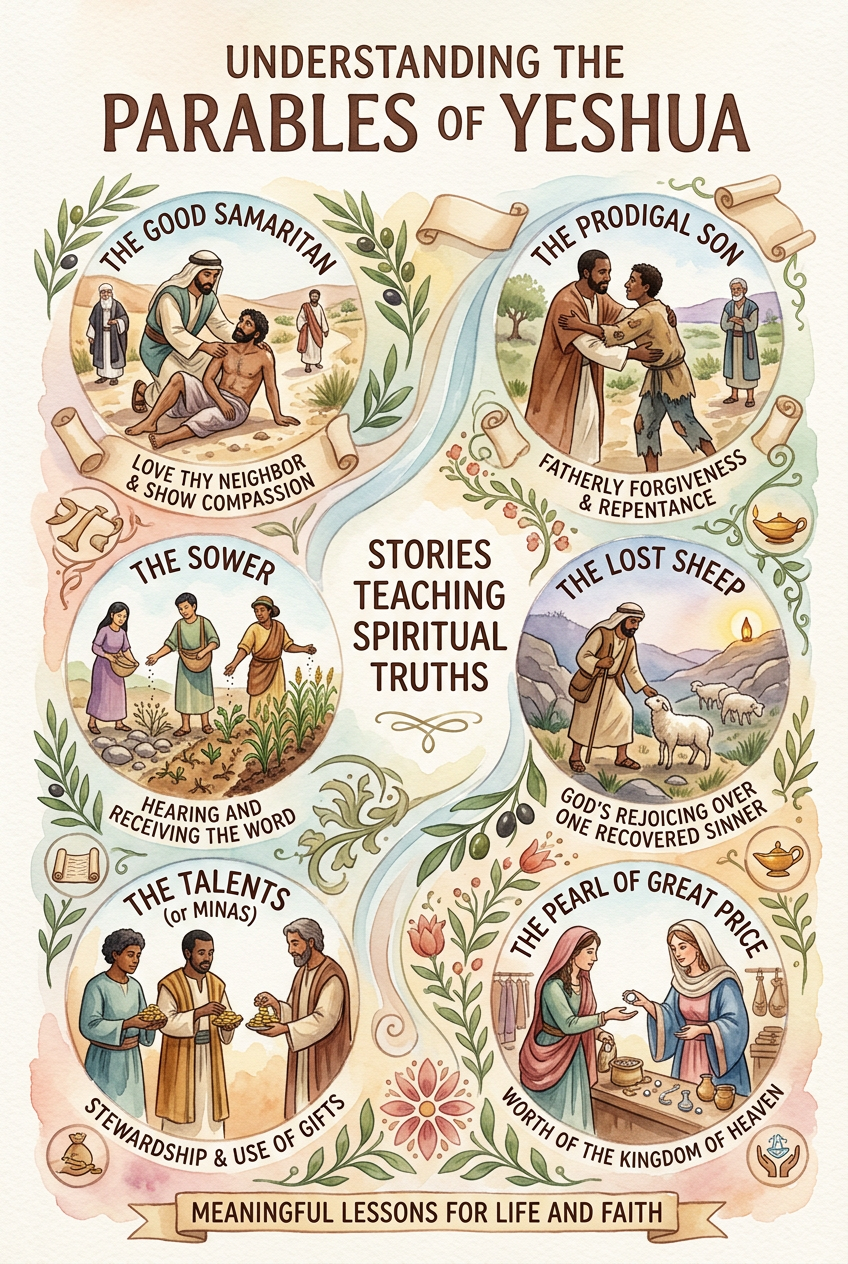
\includepdf[pages=1, fitpaper=false, width=\paperwidth, height=\paperheight, , keepaspectratio=false]{parables.png}
